% fig 1
\begin{figure}[H]
\begin{center}
 \begin{minipage}{0.49\textwidth}
  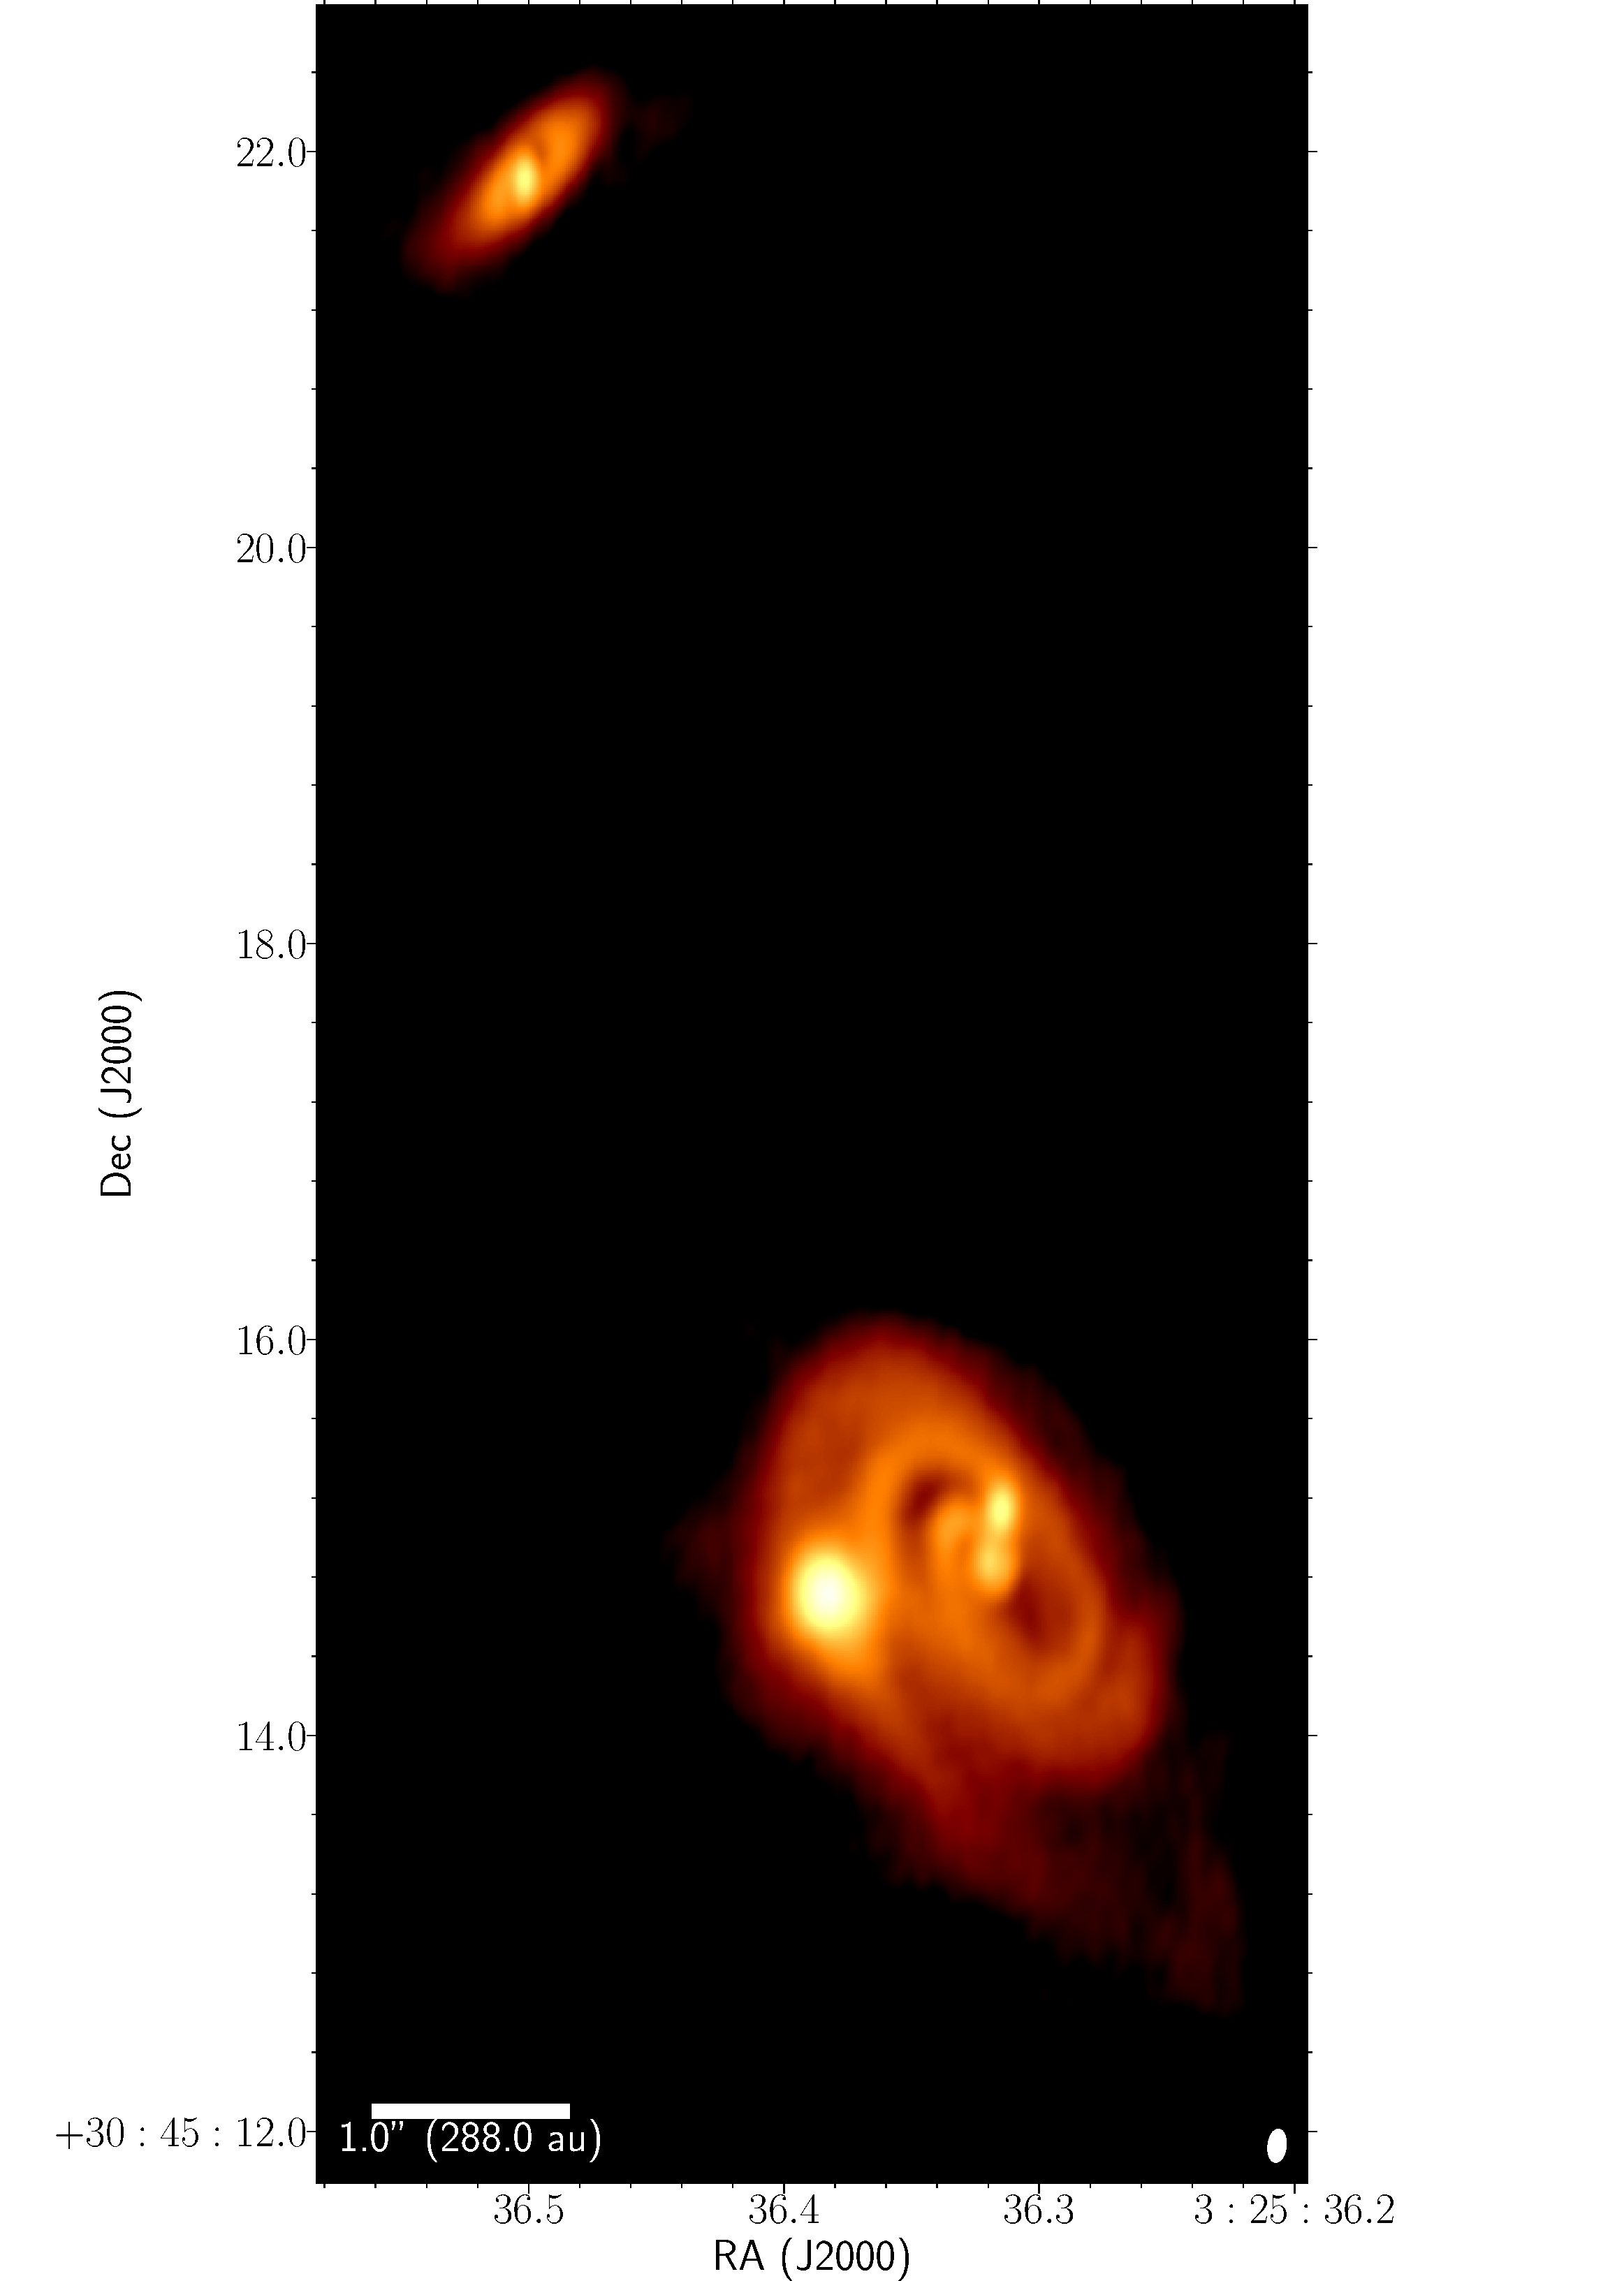
\includegraphics[width=\textwidth]{img/L1448IRS3B_cont_robust05all.pdf}
 \end{minipage}
 \begin{minipage}{0.49\textwidth}
  \vfill
  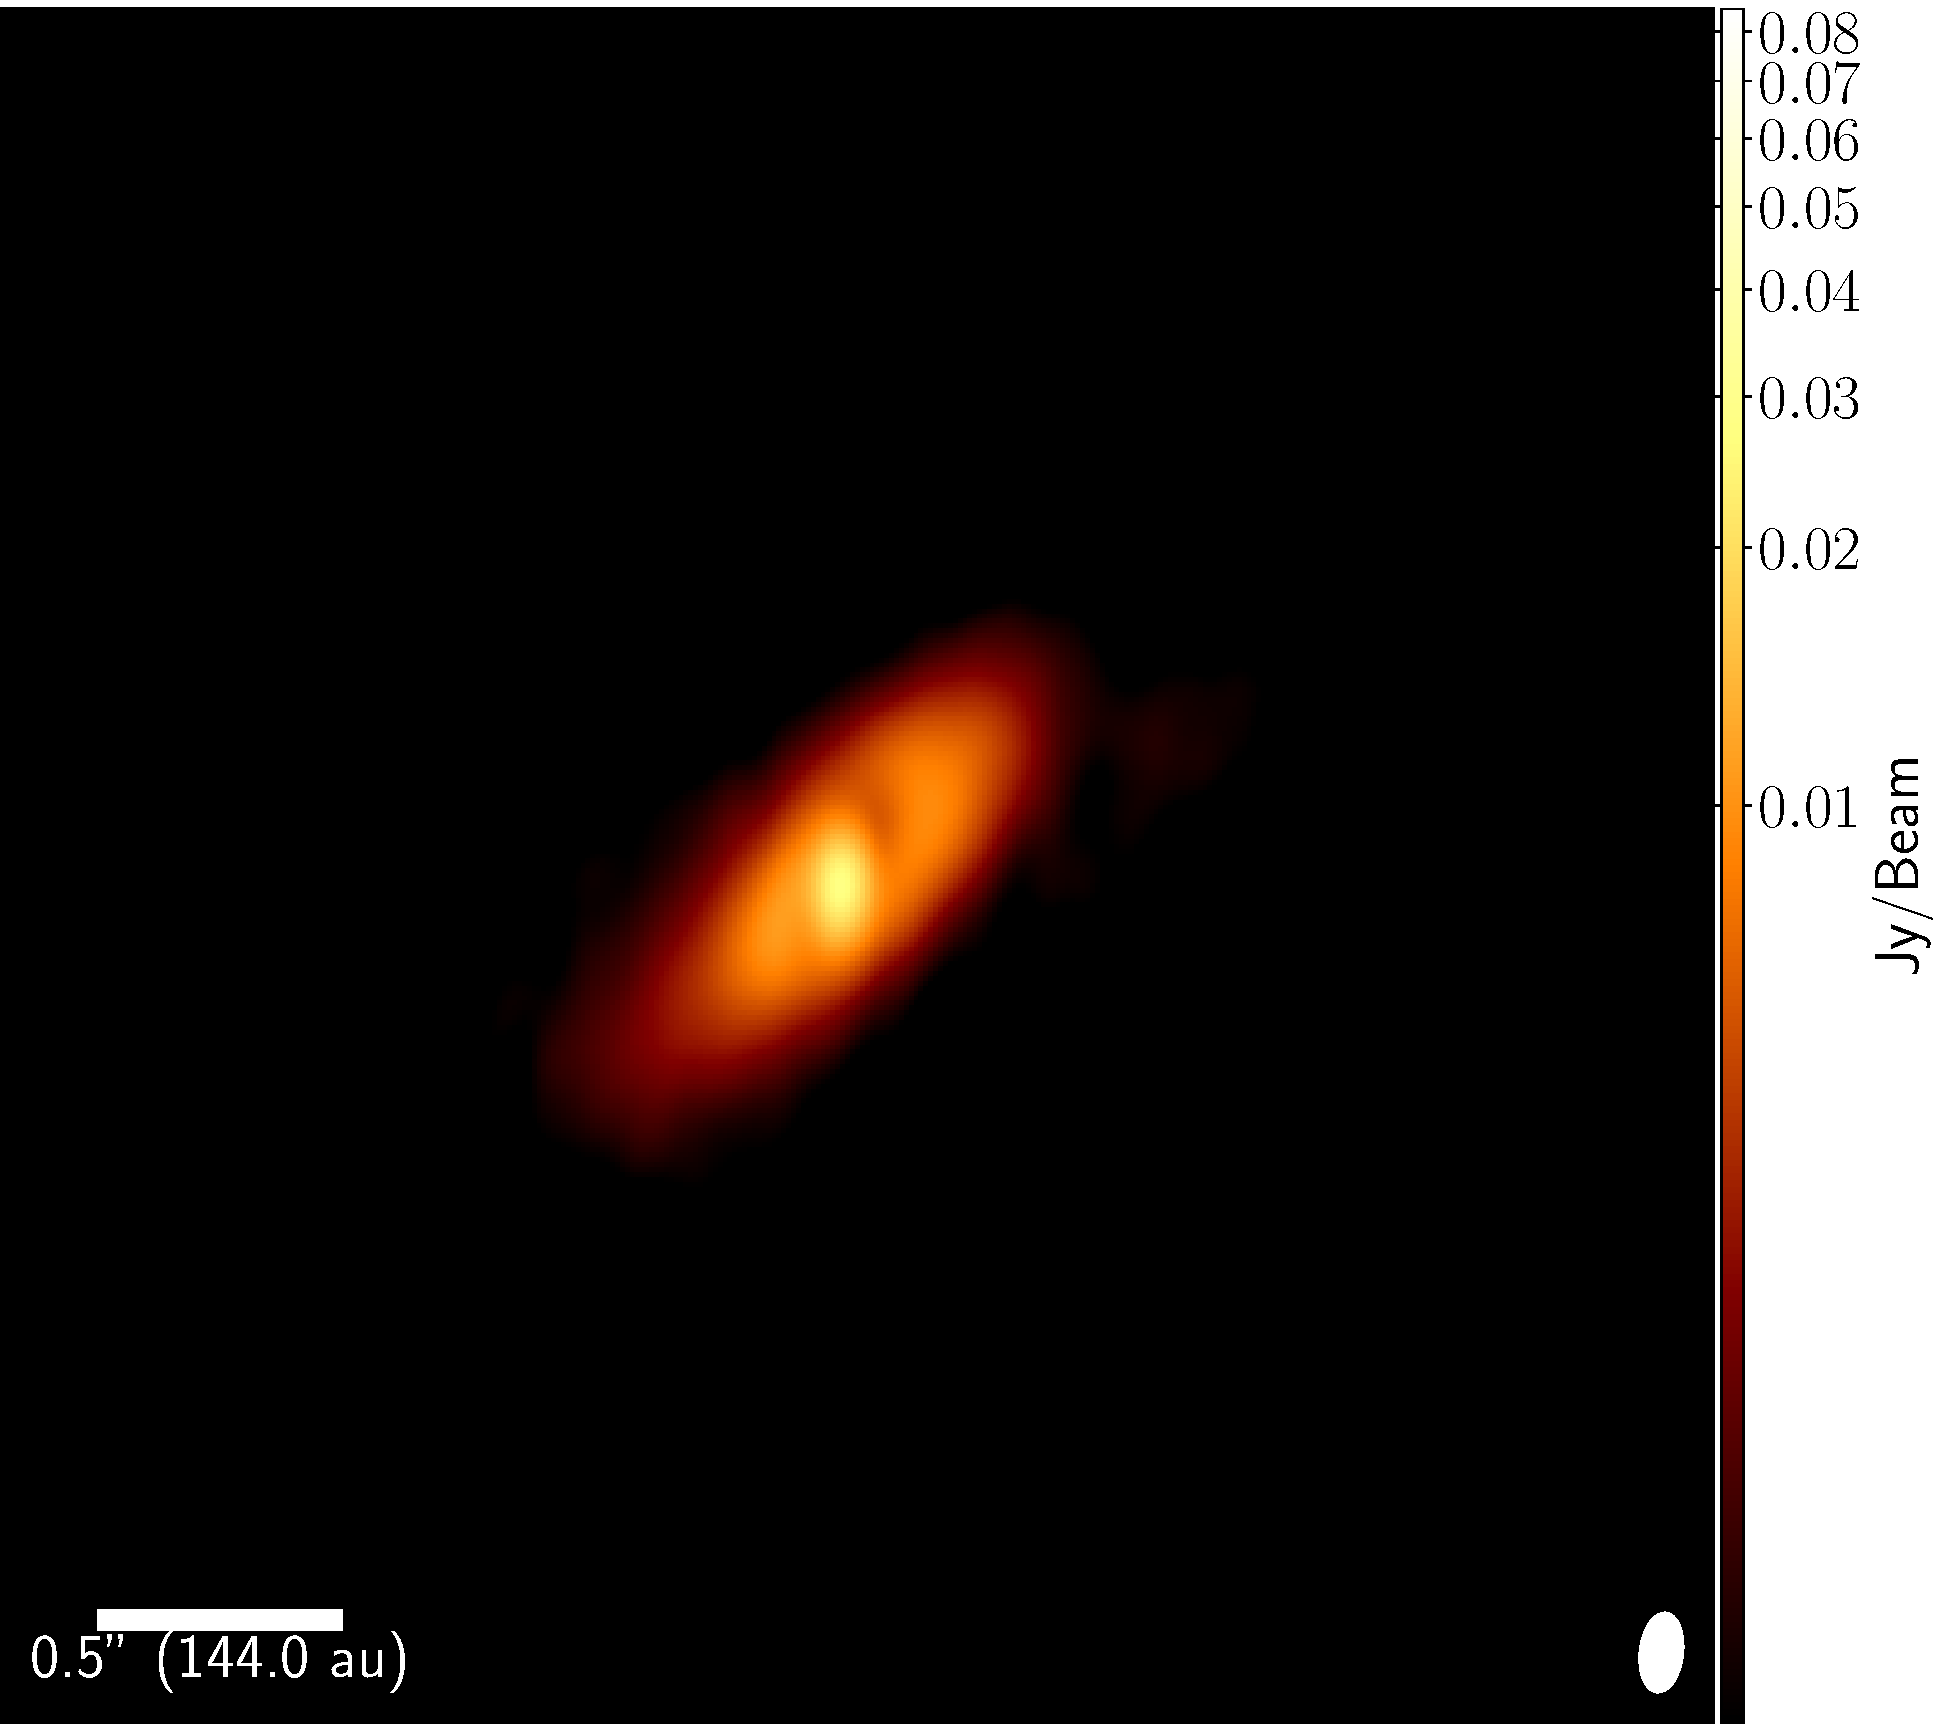
\includegraphics[width=\textwidth]{img/L1448IRS3B_cont_robust05single_uc.pdf}
  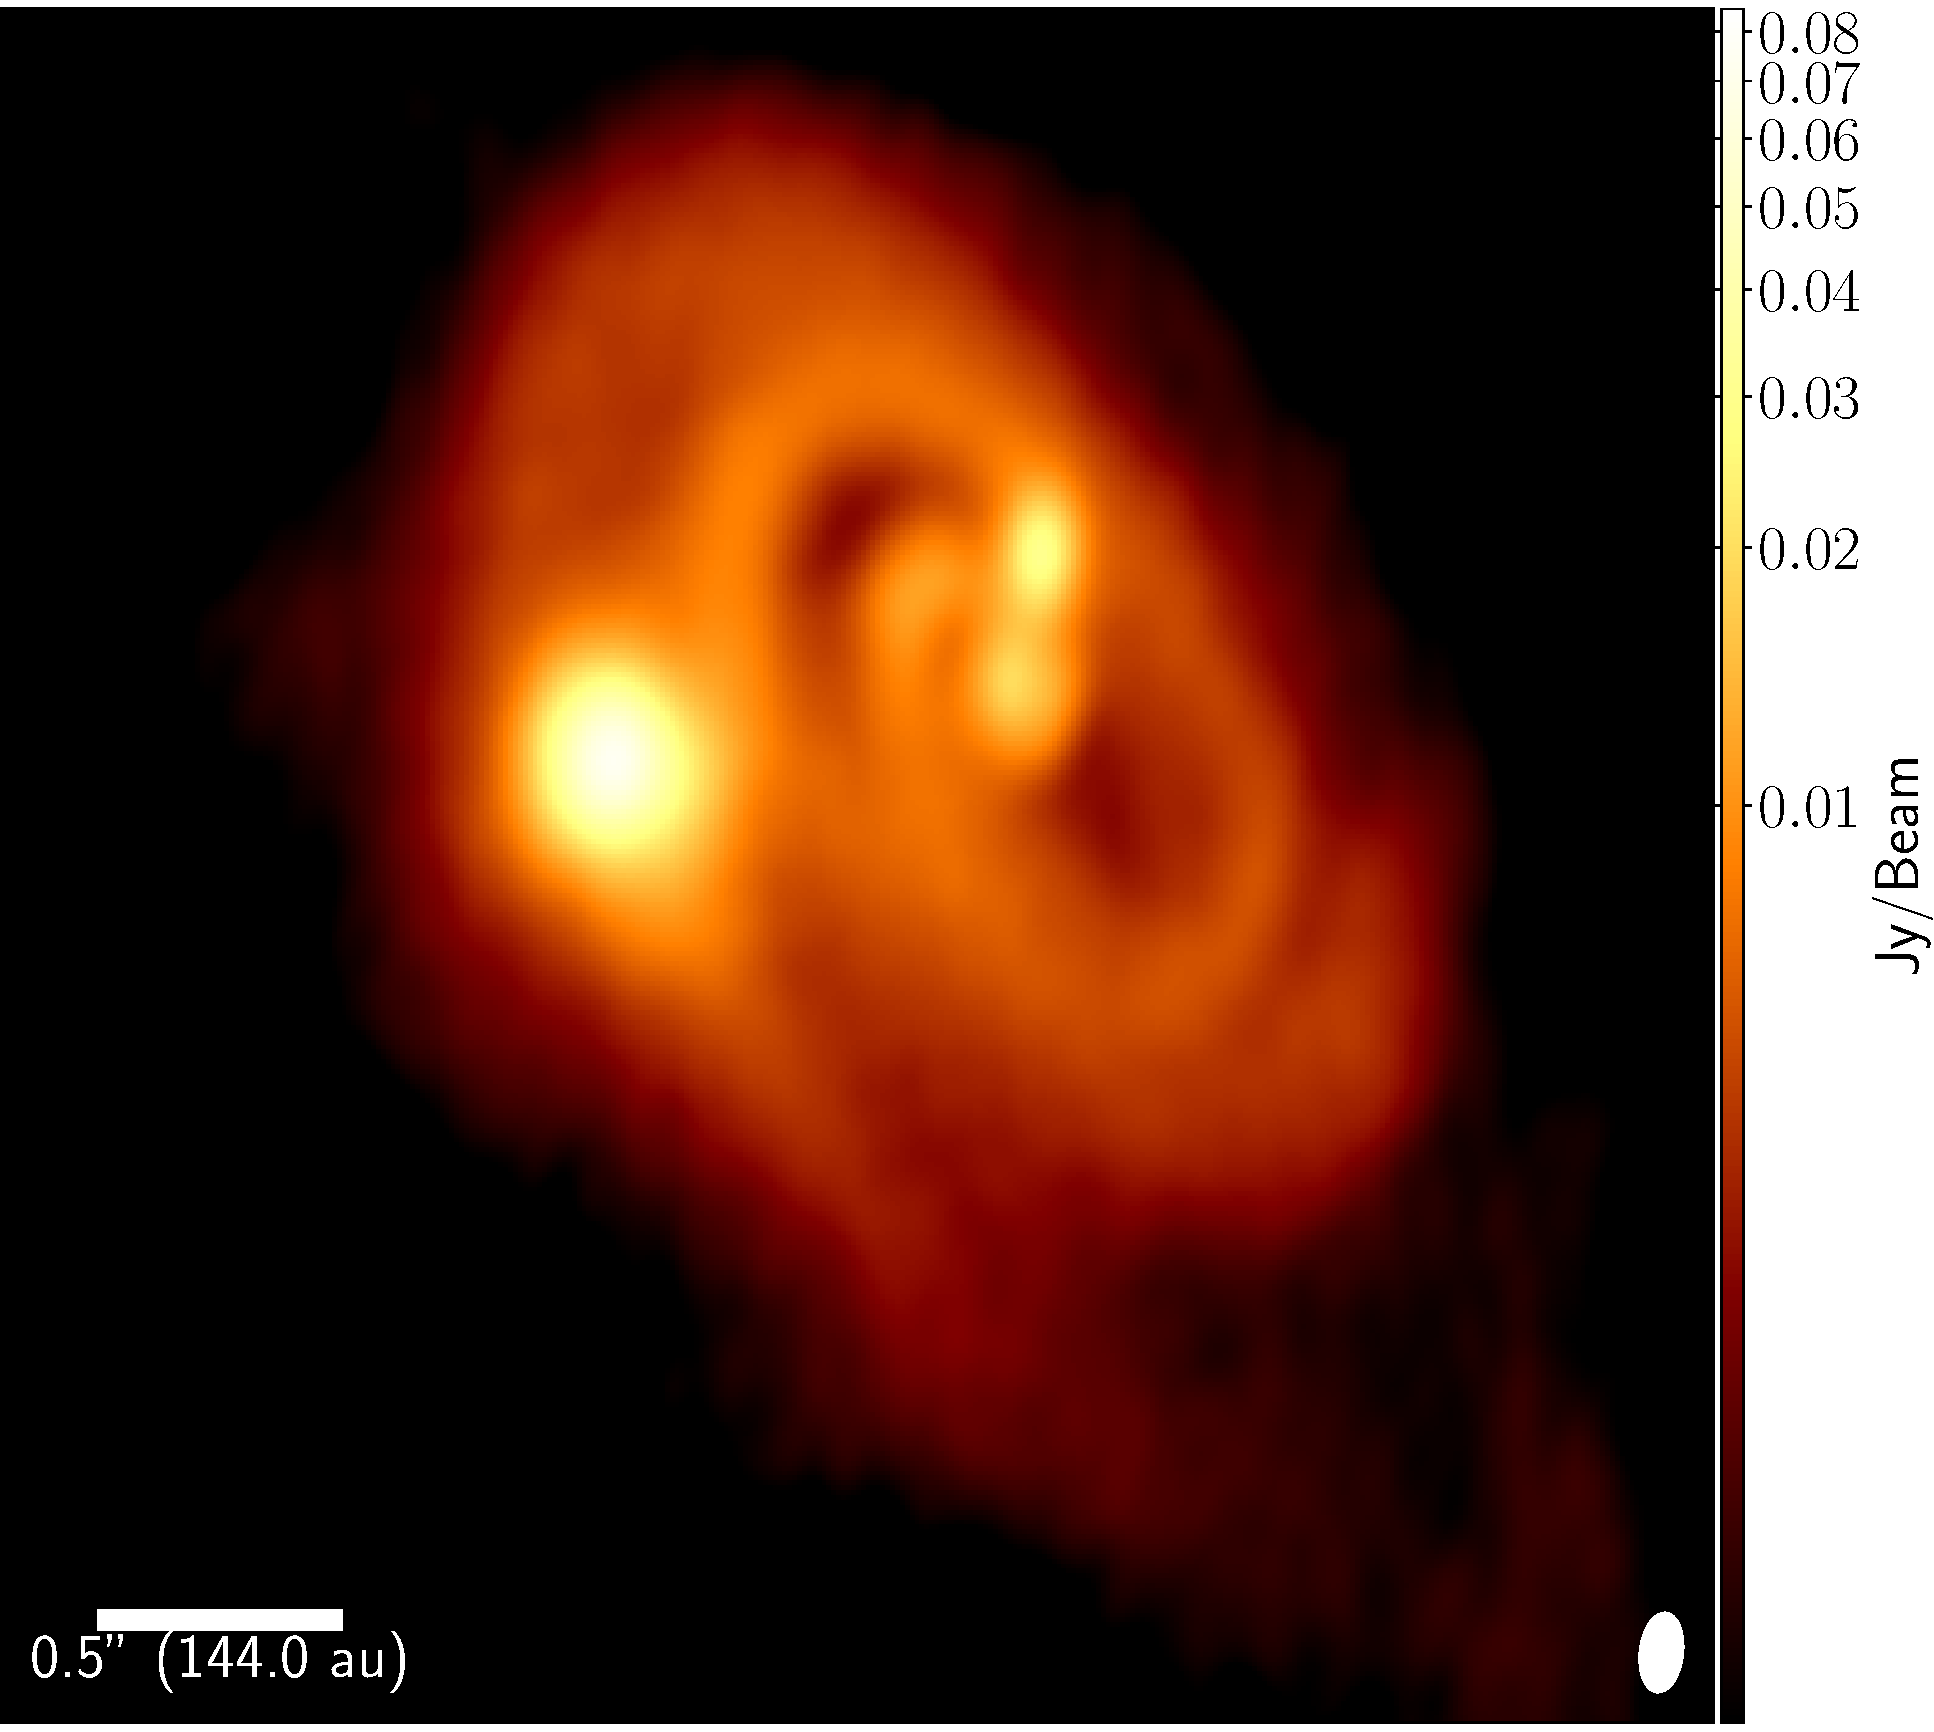
\includegraphics[width=\textwidth]{img/L1448IRS3B_cont_robust05triplet_uc.pdf}
  \vfill
 \end{minipage}
\end{center}
\caption{ALMA 879~\micron\space continuum observations of the triple protostellar system L1448 IRS3B and its wide companion IRS3A (\textbf{left}). The right panels are \ab2$\times$\space zoom-ins on IRS3B~and~IRS3A. The top right image shows the wide companion, IRS3A, (d\ab7\farcs9$\approx$2300~au), featuring possible spiral structure. The bottom right image zooms in on the proto-multiple system, IRS3B. The inner binary is separated by 0\farcs25 (75~au) and has a spiral circum-binary disk with the embedded source \ab0\farcs8 (230~au) away from the binary within one of the arms. The beam size of each panel is shown in lower right (\contbeam).}\label{fig:contimage}
\end{figure}



% Figure 17
\begin{figure}[H]
\begin{center}
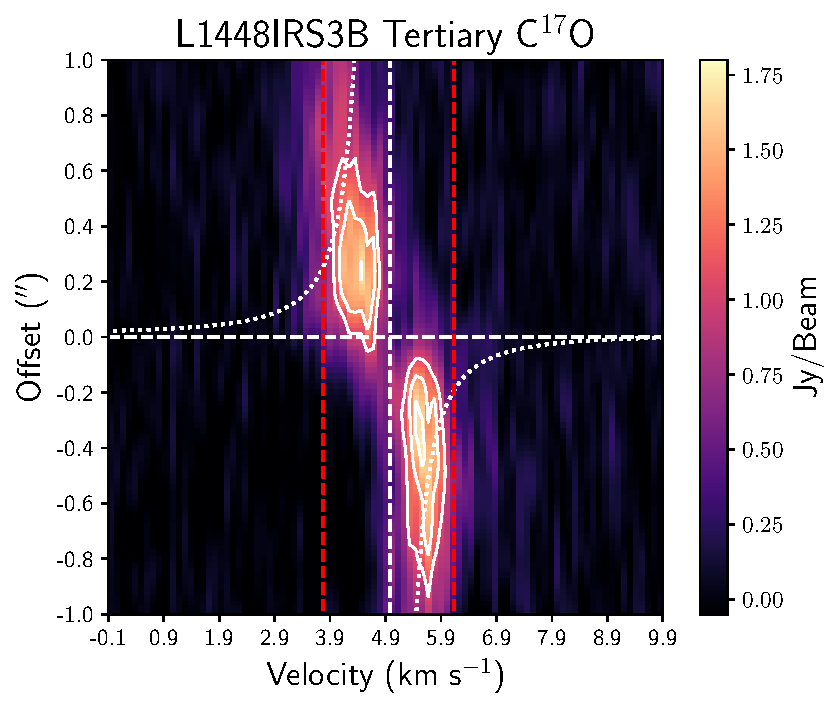
\includegraphics[width=0.5\textwidth]{img/PV-Diagram_L1448IRS3B_C17O_image_taper1500k_image_tertiary31.pdf}
\end{center}
\caption{PV-diagram of \cso\space toward IRS3B-c, the tertiary. The white lines corresponding to a Keplerian curve of a 0.2~\solm\space protostellar source. These fits place an upper limit to the mass of the tertiary companion to $<$0.2~\solm, since any larger mass and we would expect to see emission extending to high velocity, indicating the tertiary would be affecting disk kinematics. The red dashed lines indicate the maximum Keplerian velocities at the radius of IRS3B-c in the rotating disk corresponding to the 1.15~\solm\space mass of the central potential. Emission outside of these bounds could be due to the tertiary affecting disk kinematics, but from this analysis, we cannot detect an obvious effect of the tertiary on the disk kinematics. The white/black contours trace regions starting from 14$\sigma$ at 4$\sigma$\space intervals, where $\sigma\approx$0.1~Jy~beam$^{-1}$.}\label{fig:l1448irs3b_c17o_pv_tert}
\end{figure}



% Figure 6
\begin{figure}[H]
\begin{center}
   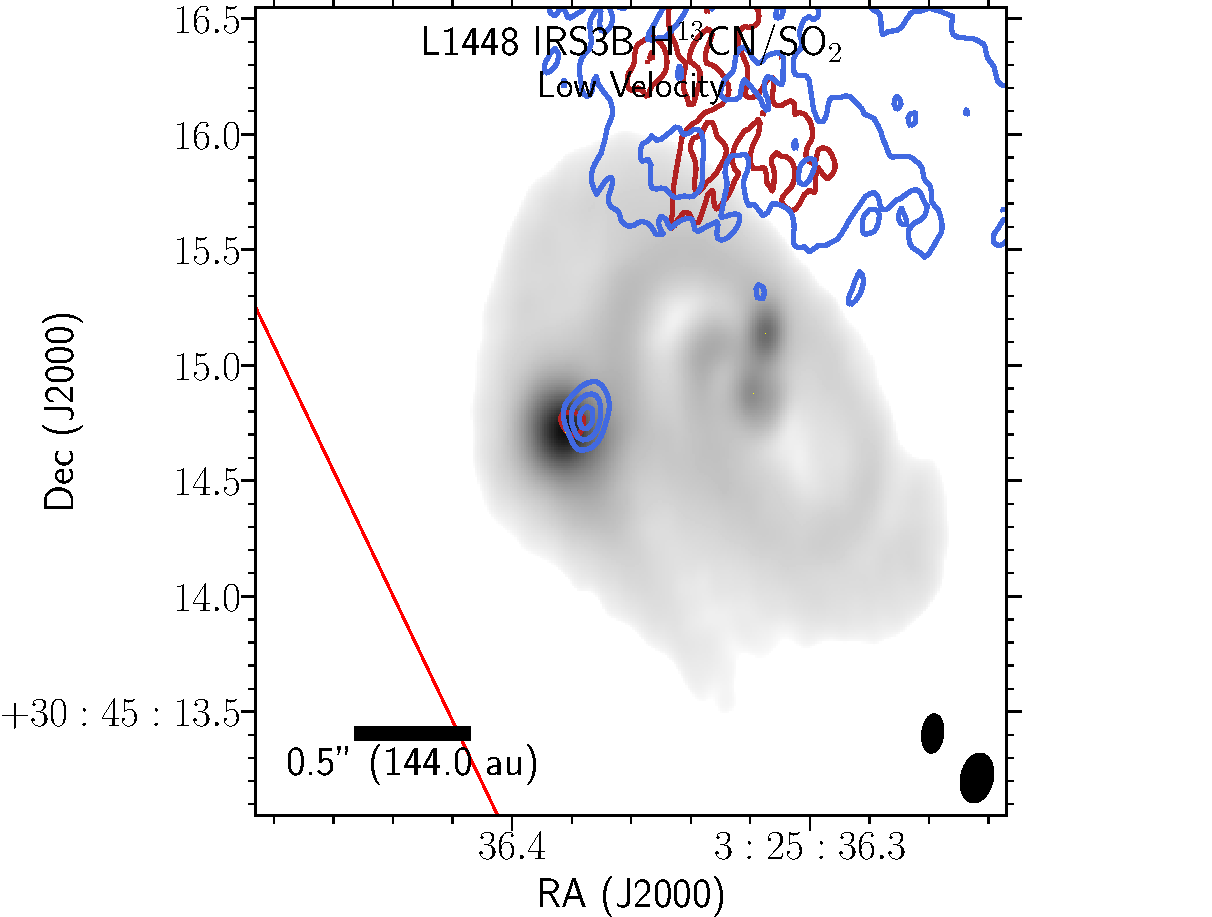
\includegraphics[width=0.33\textwidth]{img/L1448IRS3B_H13CN_clean_image_2_binned__low.pdf}
   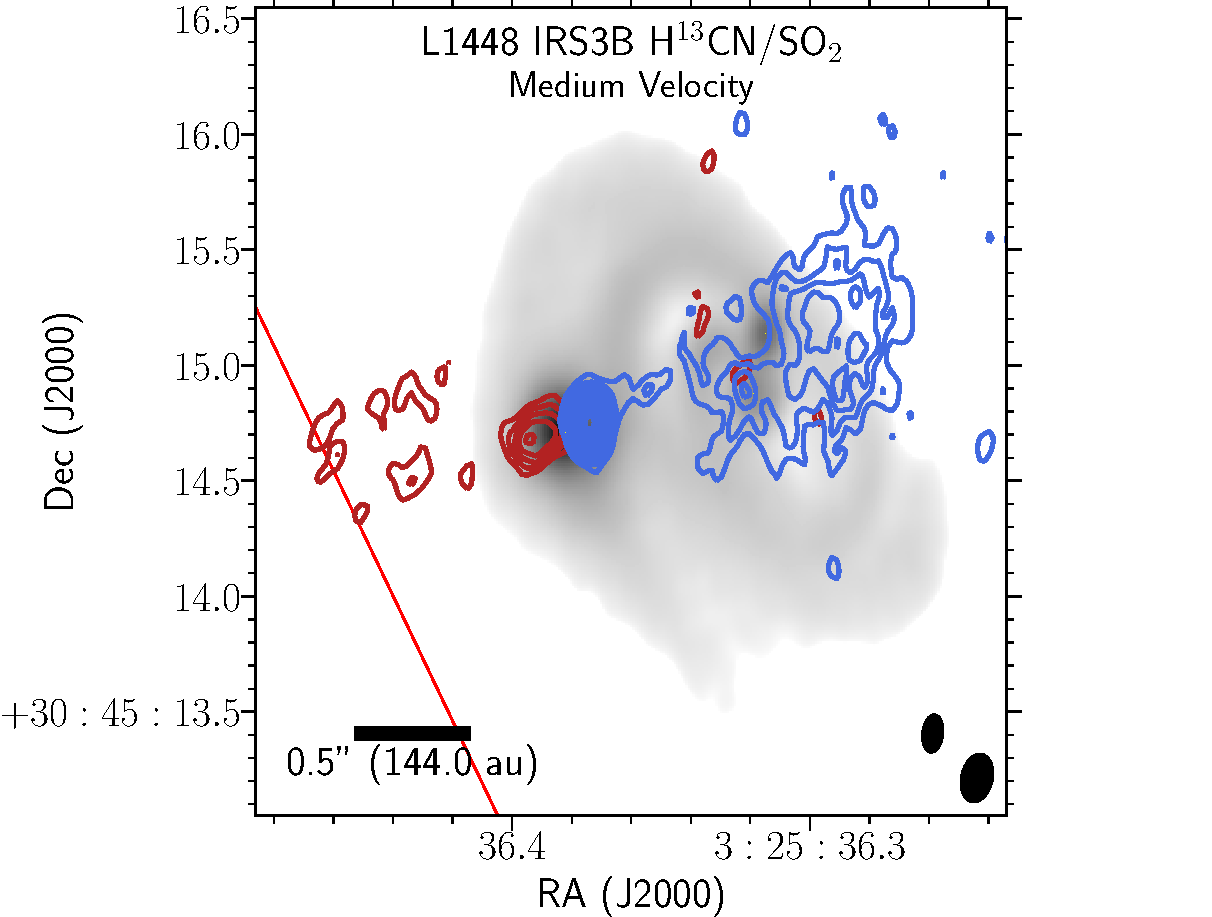
\includegraphics[width=0.33\textwidth]{img/L1448IRS3B_H13CN_clean_image_2_binned__med.pdf}
   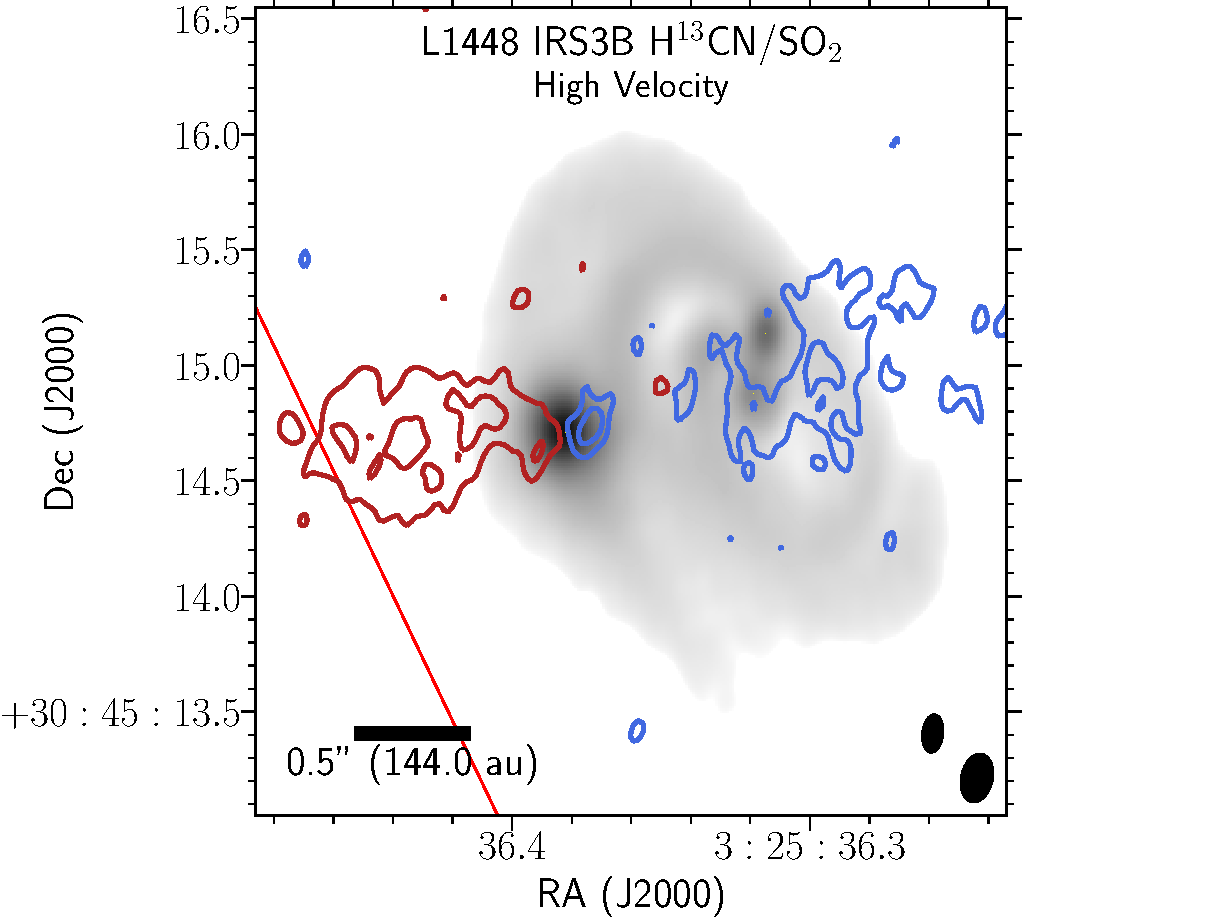
\includegraphics[width=0.33\textwidth]{img/L1448IRS3B_H13CN_clean_image_2_binned__high.pdf} % h13cn
\end{center}
   \caption{\htcn/\sot\space moment 0 map towards IRS3B, appears to trace near the outflow launch location from the tertiary, IRS3B-c. There is pretty large asymmetry in the velocity channels covered by the red and blue-shifted emission. The panels correspond to low, medium, and high velocity ranges. \textbf{Low Velocity:} velocity ranges 5.2$\rightarrow$7.2~\kms (4$\rightarrow$4.8~\kms), contours start at 5(5)$\sigma$ and iterate by 2(5)$\sigma$ with the 1$\sigma$~level starting at 0.0025(0.0021)~Jy~beam$^{-1}$ for the red(blue) channels respectively. \textbf{Medium Velocity:} velocity ranges 7.2$\rightarrow$9.2~\kms (3.2$\rightarrow$4~\kms), contours start at 5(5)$\sigma$ and iterate by 2(2)$\sigma$ with the 1$\sigma$~level starting at 0.0016(0.0016)~Jy~beam$^{-1}$ for the red(blue) channels respectively. \textbf{High Velocity:} velocity ranges 9.2$\rightarrow$11.2~\kms (1.6$\rightarrow$3.2~\kms), contours start at 4(4)$\sigma$ and iterate by 3(3)$\sigma$ with the 1$\sigma$~level starting at 0.0021(0.0021)~Jy~beam$^{-1}$ for the red(blue) channels respectively. The \htcn\space synthesized beam (\htcnbeam) is the bottom-right most ellipse on each of the panels and the continuum synthesized beam (\contbeam) is offset diagonally.}\label{fig:irs3bh13cnmoment}
\end{figure}




% Figure 19
\begin{figure}[H]
\begin{center}
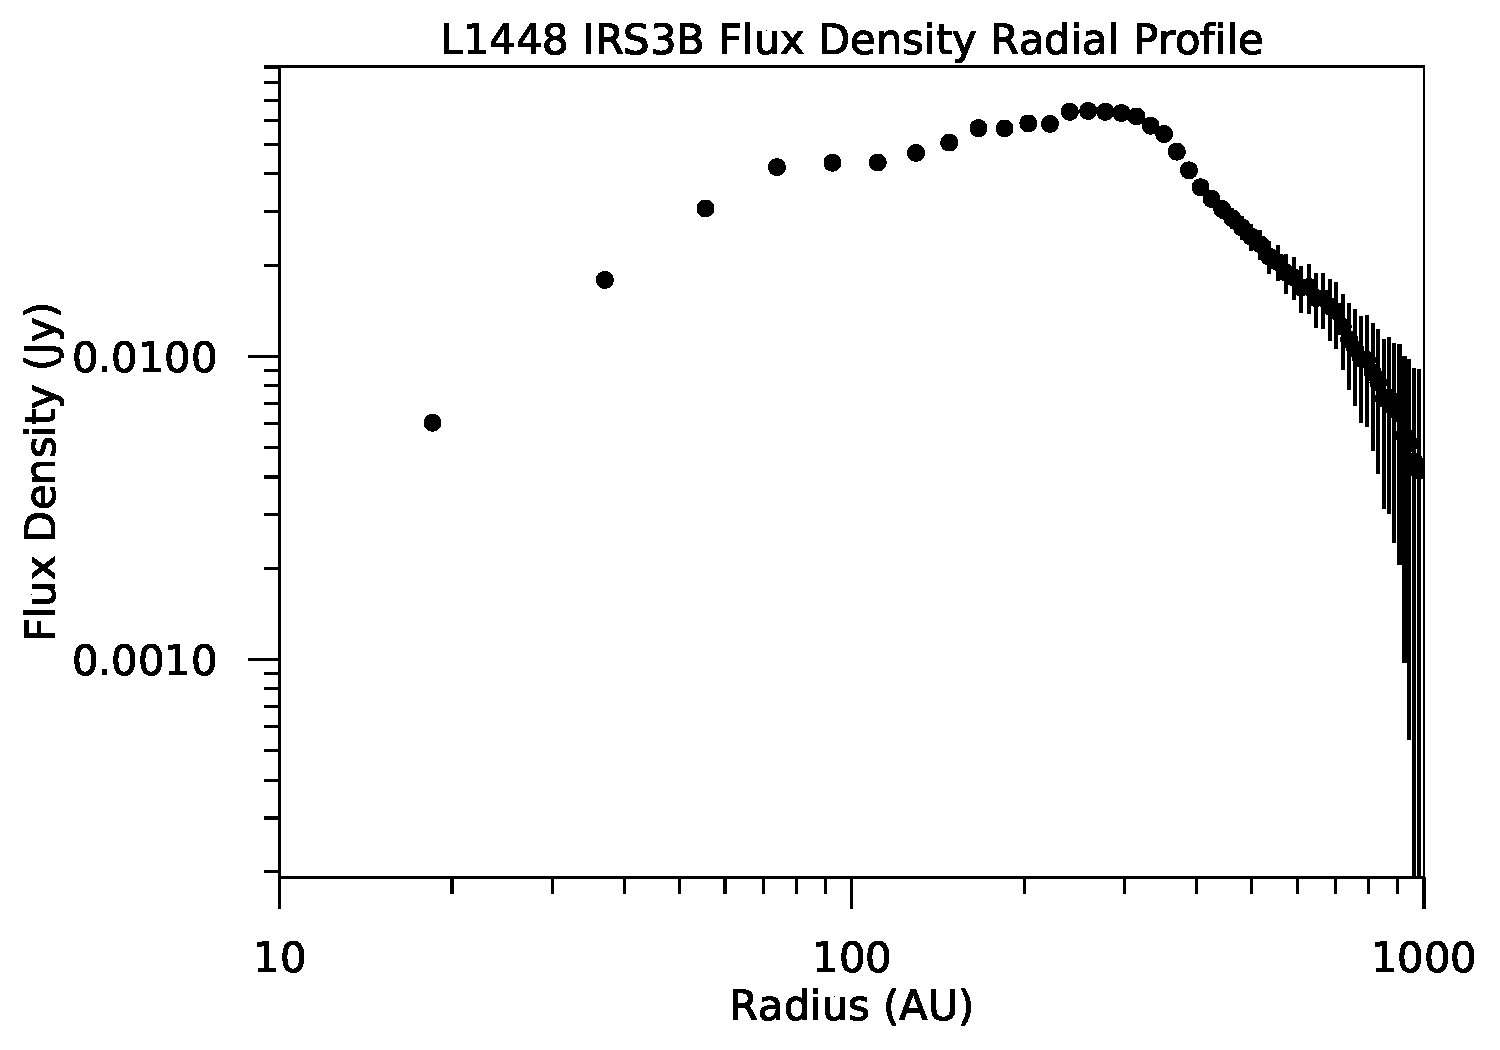
\includegraphics[width=0.49\textwidth]{img/L1448N-dgr-linear-intensity-c17o_cont.pdf}
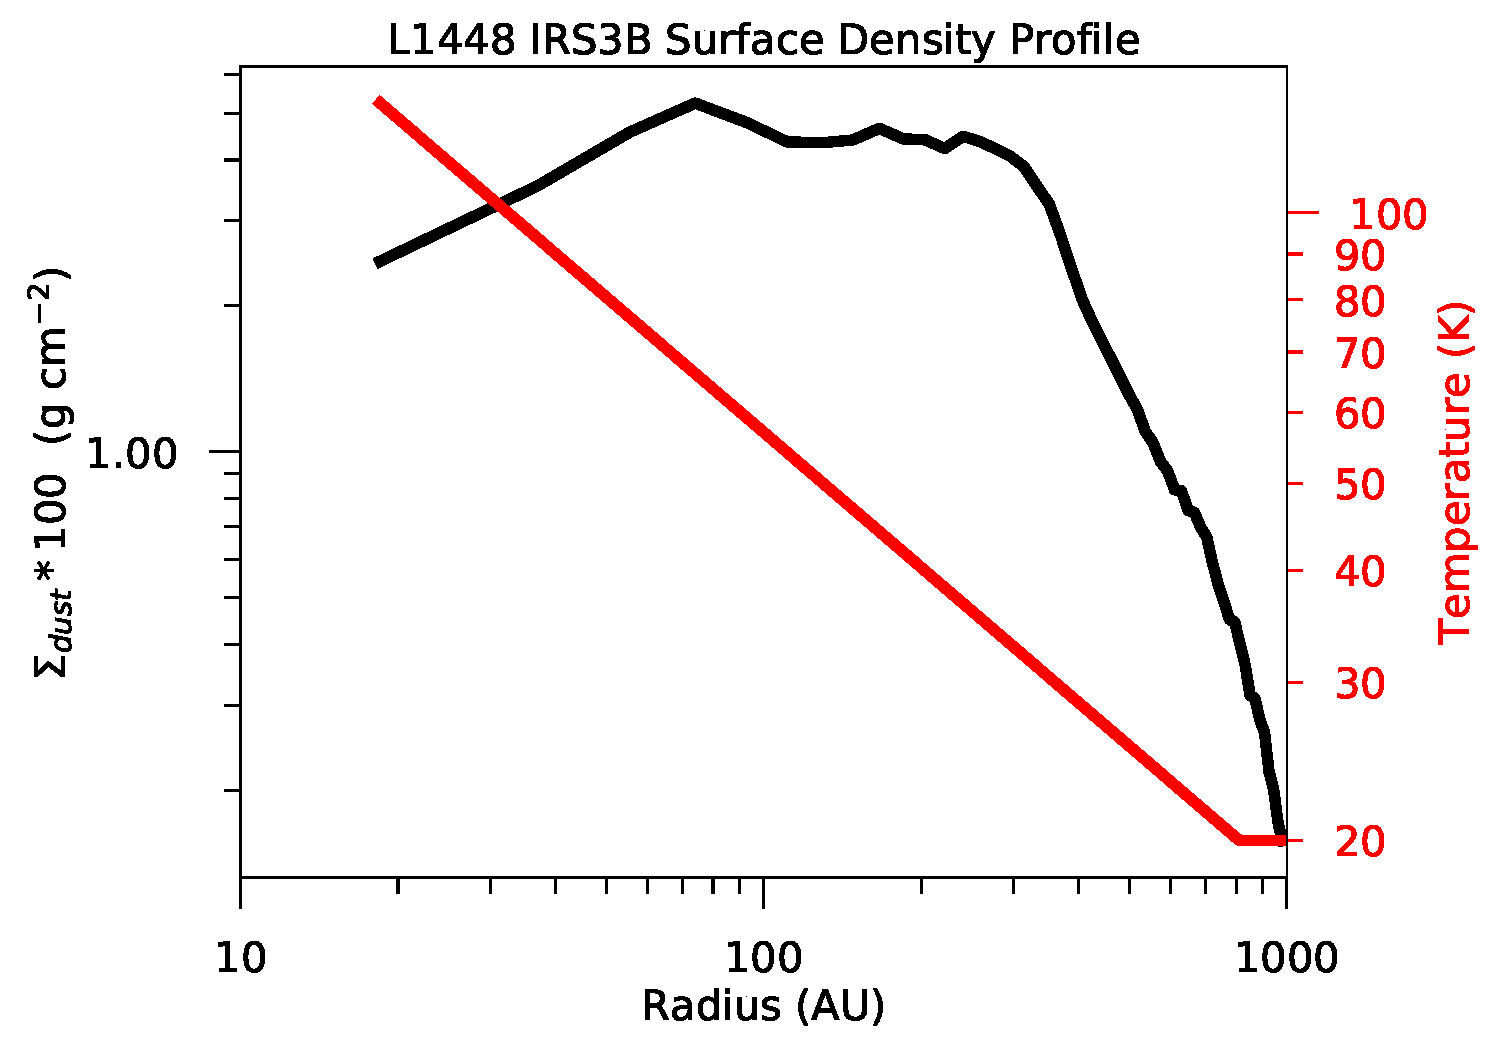
\includegraphics[width=0.49\textwidth]{img/L1448N-dustgas-surface-density-loglog.pdf}
\end{center}
\caption{The left plot is the continuum flux density radial profile of IRS3B. The right plot is the deprojected radial surface density profile of the dust continuum in black , while the red line is the radial temperature profile of the disk. The temperature profile is $\propto\text{R}^{-0.5}$ and is scaled such that at 100~AU is described via (30~K)$\times(L_{*}$/\lsun)$^{0.25}\approx40.1$~K.}\label{fig:surfacedensity}
\end{figure}

% figure 20
\begin{figure}[H]
\begin{center}
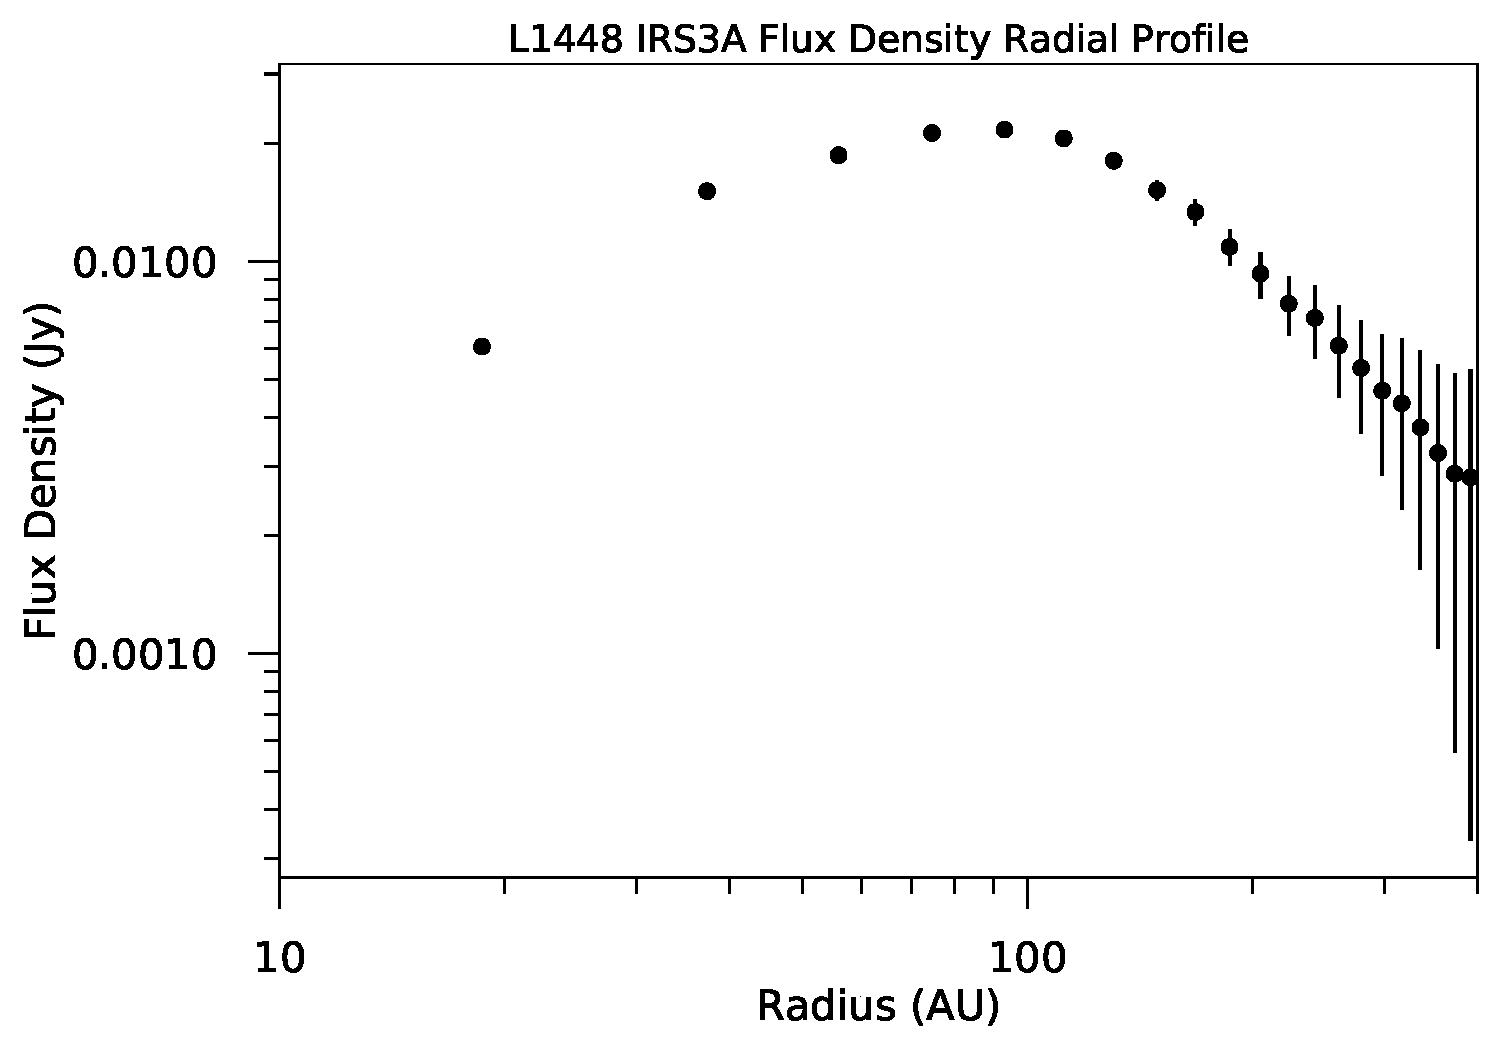
\includegraphics[width=0.49\textwidth]{img/L1448N-intensity-rad-xsec-cont_robust-05_wide.pdf}
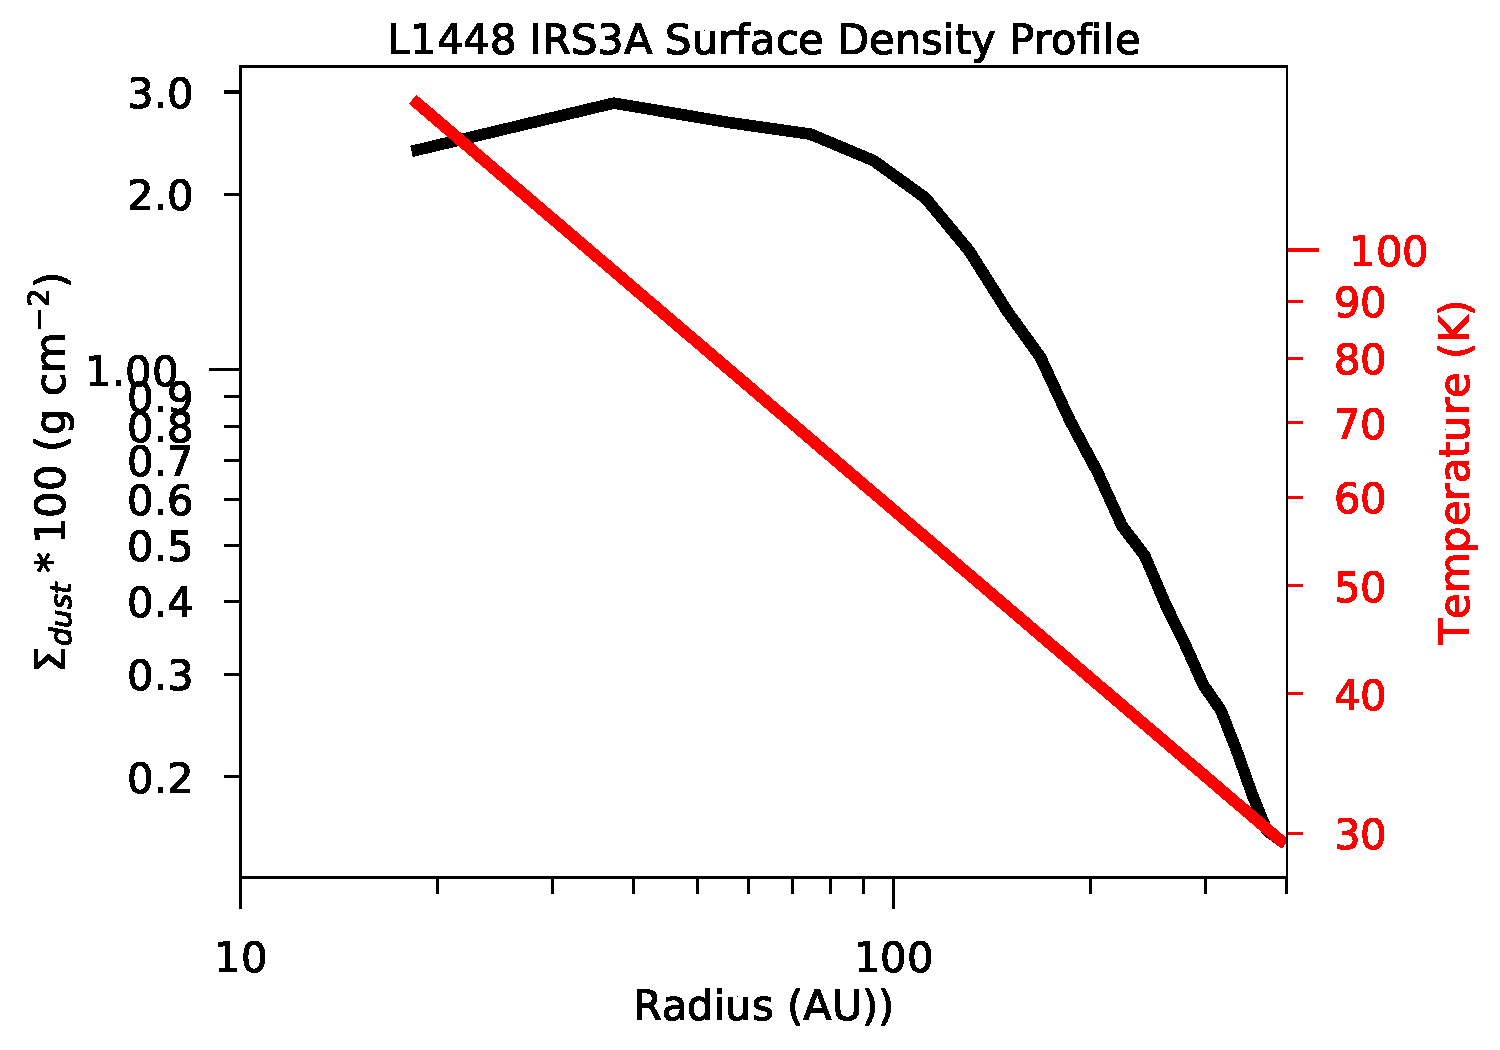
\includegraphics[width=0.49\textwidth]{img/L1448N-surface-density-lograd-xsec-cont_robust-05_wide.pdf}
\end{center}
\caption{The left plot is the continuum flux density radial profile of IRS3A. The right plot is the radial surface density profile of the dust continuum in black, while the red line is the radial temperature profile of the disk. The temperature profile is $\propto\text{R}^{-0.5}$ and is scaled such that at 100~AU is described via (30~K)$\times(L_{*}$/\lsun)$^{0.25}\approx53.1$~K.}\label{fig:irs3asurfacedensity}
\end{figure}



% Figure 17
\begin{figure}[H]
\begin{center}
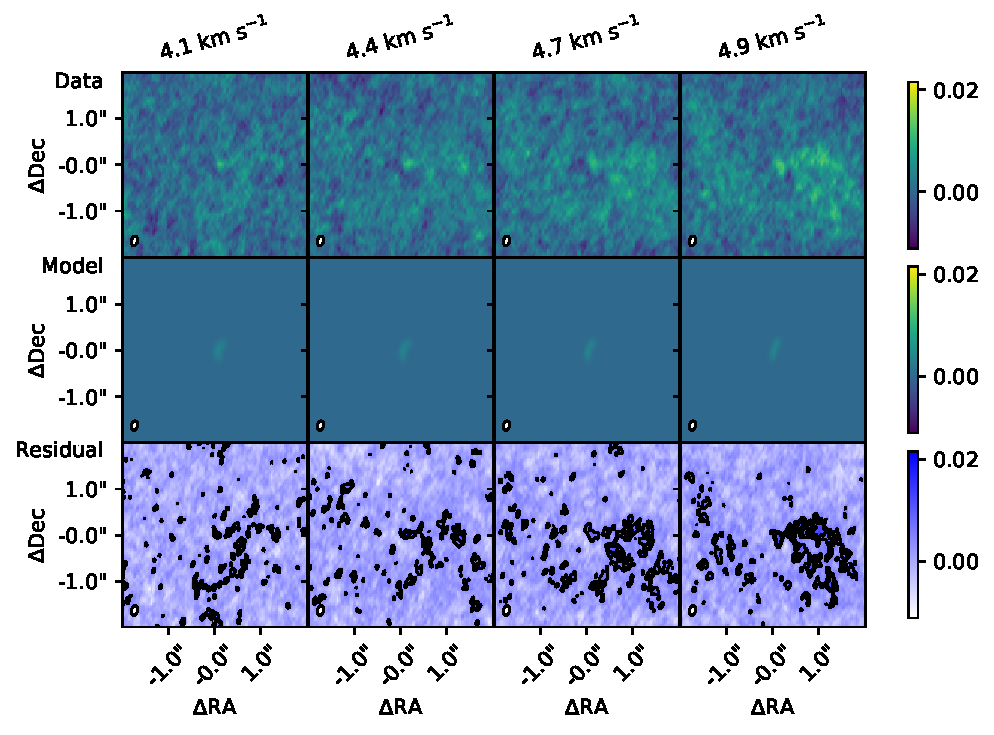
\includegraphics[width=0.49\textwidth]{img/Channelplot_h13cnplotblue_H13CN.pdf}
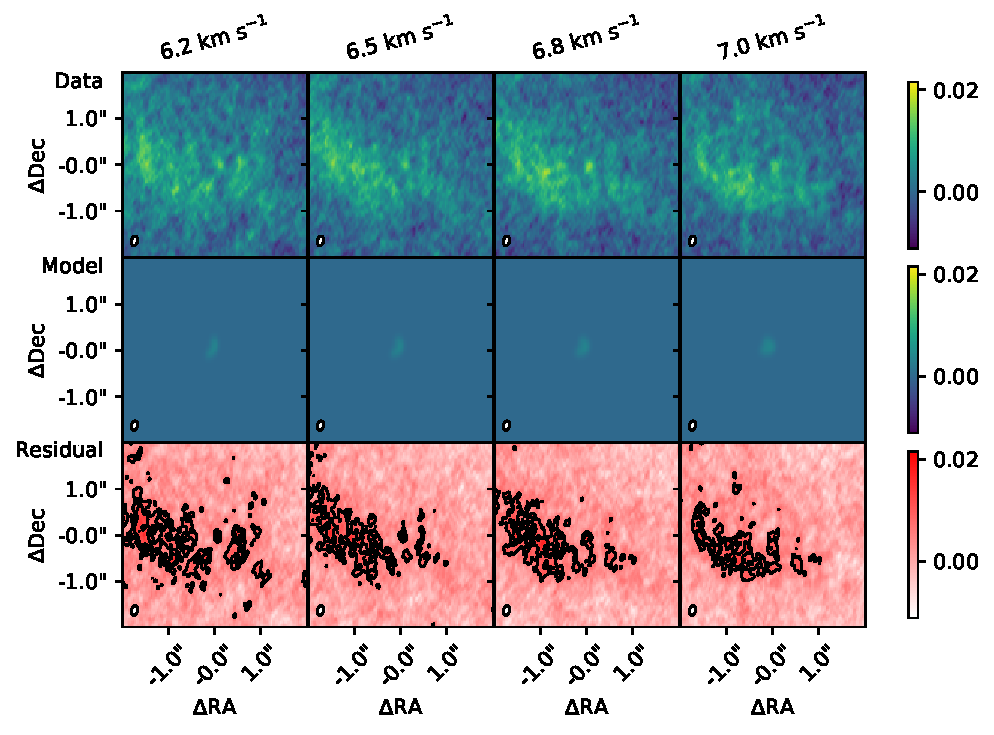
\includegraphics[width=0.49\textwidth]{img/Channelplot_h13cnplotred_H13CN.pdf}
\end{center}
\caption{IRS3A Kinematic Model comparison, similar to Figure~\ref{fig:c17o_res}. System velocity is \ab5.2~km~s$^{-1}$. There is residual emission at scales much larger than the continuum disk, especially prevalent near the system velocity, likely due to large scale emission from the cloud that is not included in the disk.}\label{fig:h13cn_res}
\end{figure}



% Figure 15
\begin{figure}[H]
\begin{center}
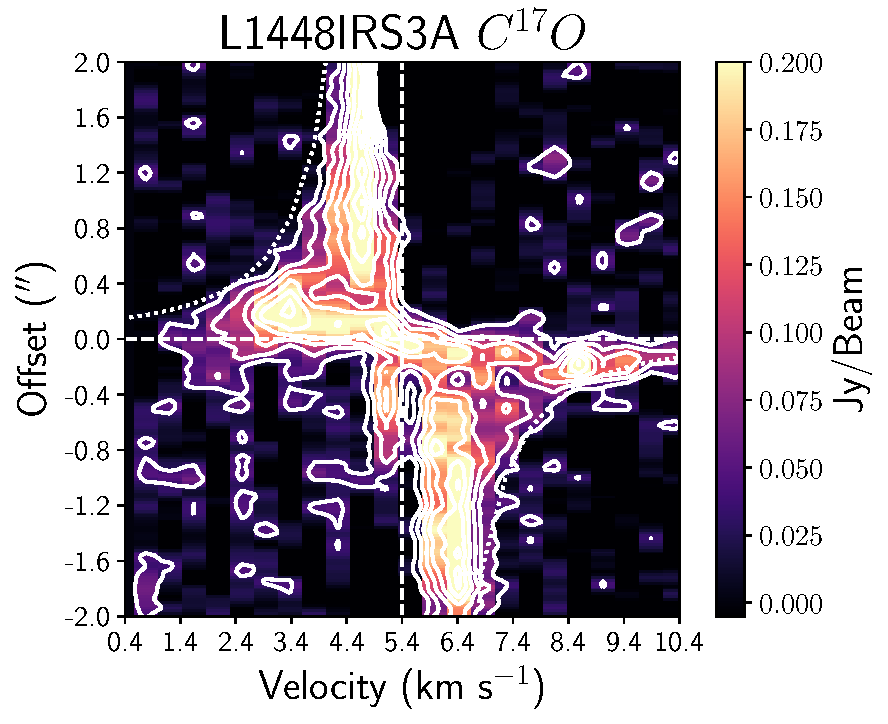
\includegraphics[width=0.33\textwidth]{img/PV-Diagram_L1448IRS3B_C17O_clean_binnedwide.pdf}
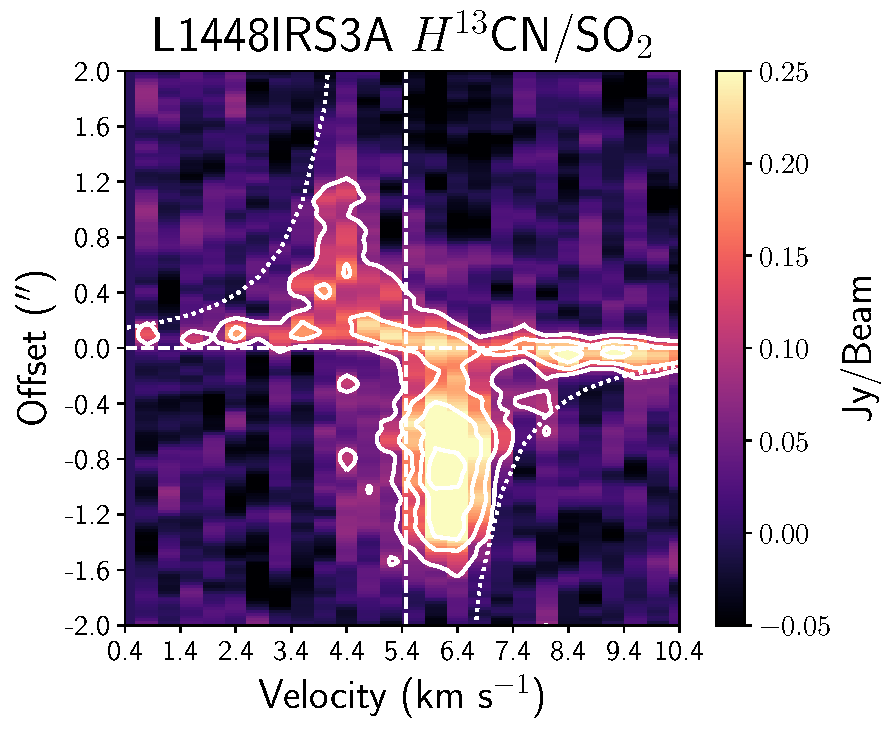
\includegraphics[width=0.33\textwidth]{img/irs3a_h13cn_pv.pdf}
   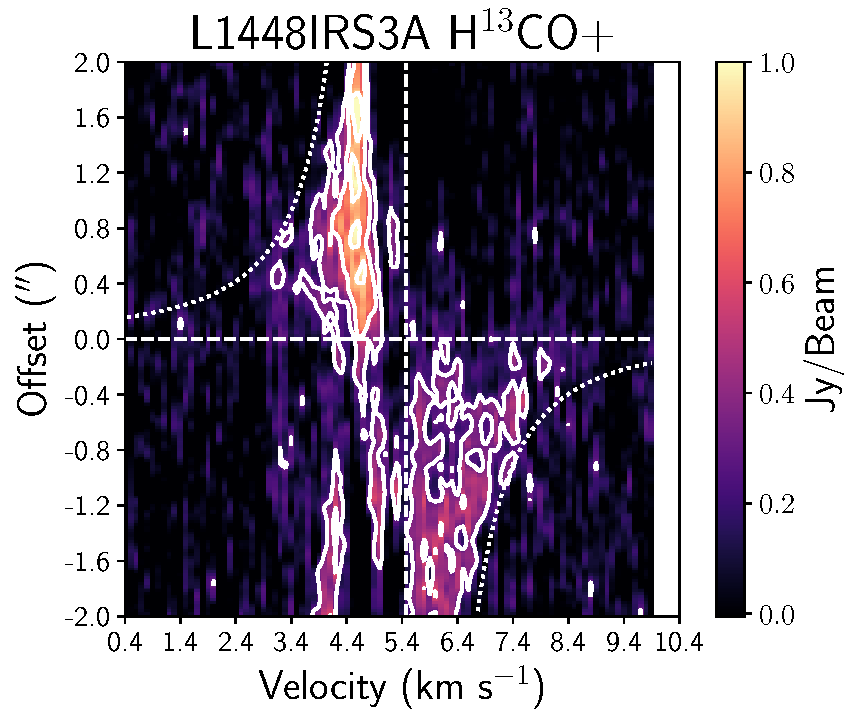
\includegraphics[width=0.33\textwidth]{img/PV-Diagram_L1448IRS3B_H13COp_image_taper1500k-wide.pdf} % h13cn
\end{center}
\caption{PV diagrams of IRS3A generated at a position angle of 125\deg. (left)\cso\space emission, with the dotted lines corresponding to 1.4~\solm. (middle) \htcn/\sot\space emission and (right)\htcop\space emission. The emission suffers from the lower spatial sampling across the source and the extended, resolved-out emission from the IRS3B$+$A envelope/core. Similarly, strong spatial integration (width of slice 0\farcs3) restrictions were placed when making the PV diagram to limit the inclusion of large-scale emission. The white contours trace regions starting from 3$\sigma$ at 2$\sigma$\space intervals, where $\sigma\approx$0.15~Jy.}\label{fig:l1448irs3a_cso_pv}
\end{figure}


% Figure 9
\begin{figure}[H]
\begin{center}
   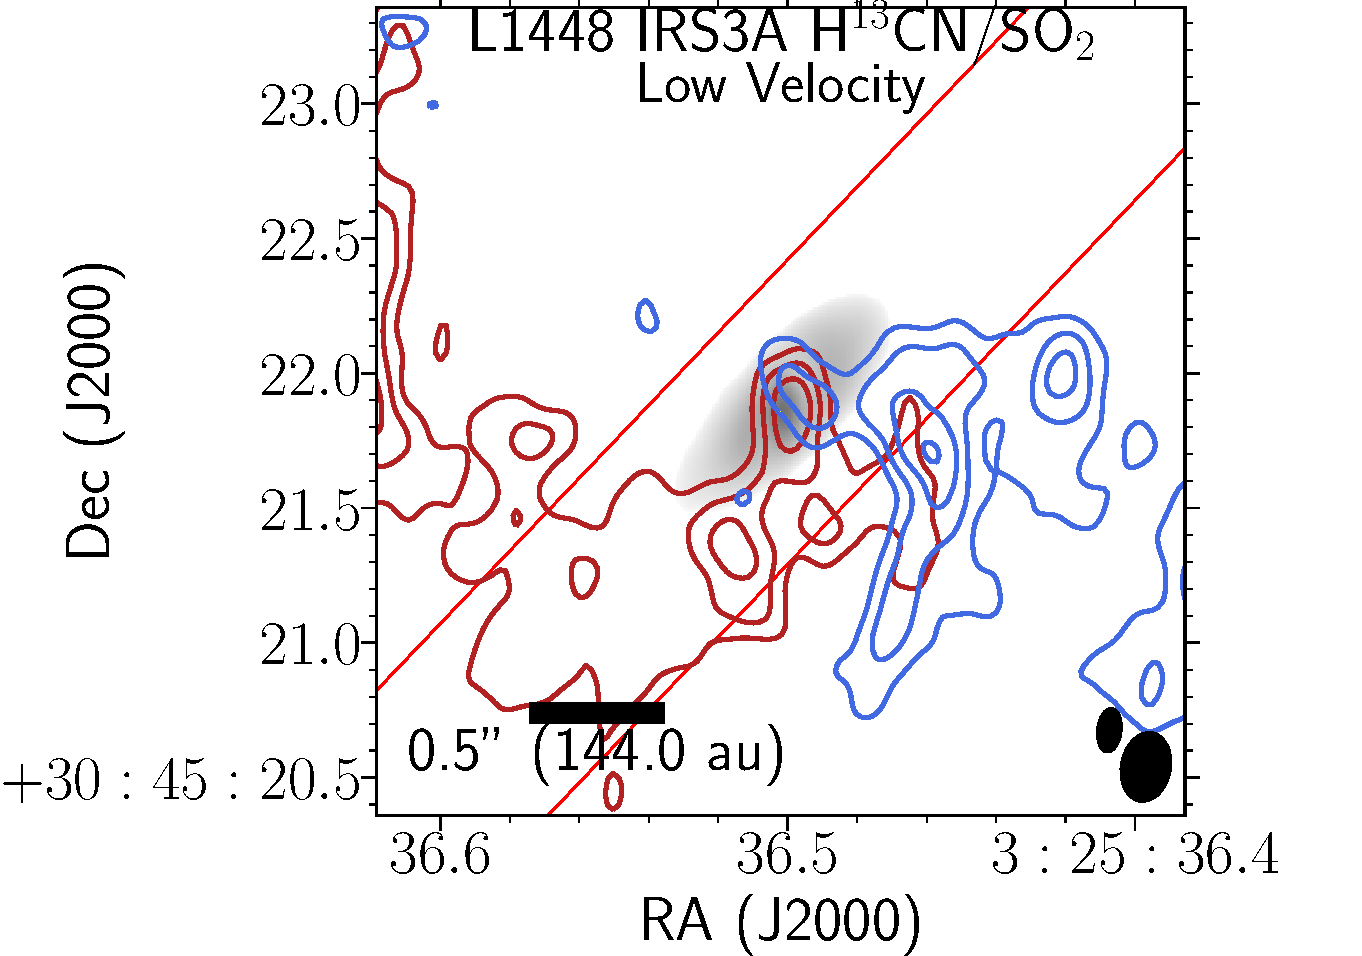
\includegraphics[width=0.33\textwidth]{img/L1448IRS3B_H13CN_image_taper1000k__-irs3alow_irs3a.pdf}
   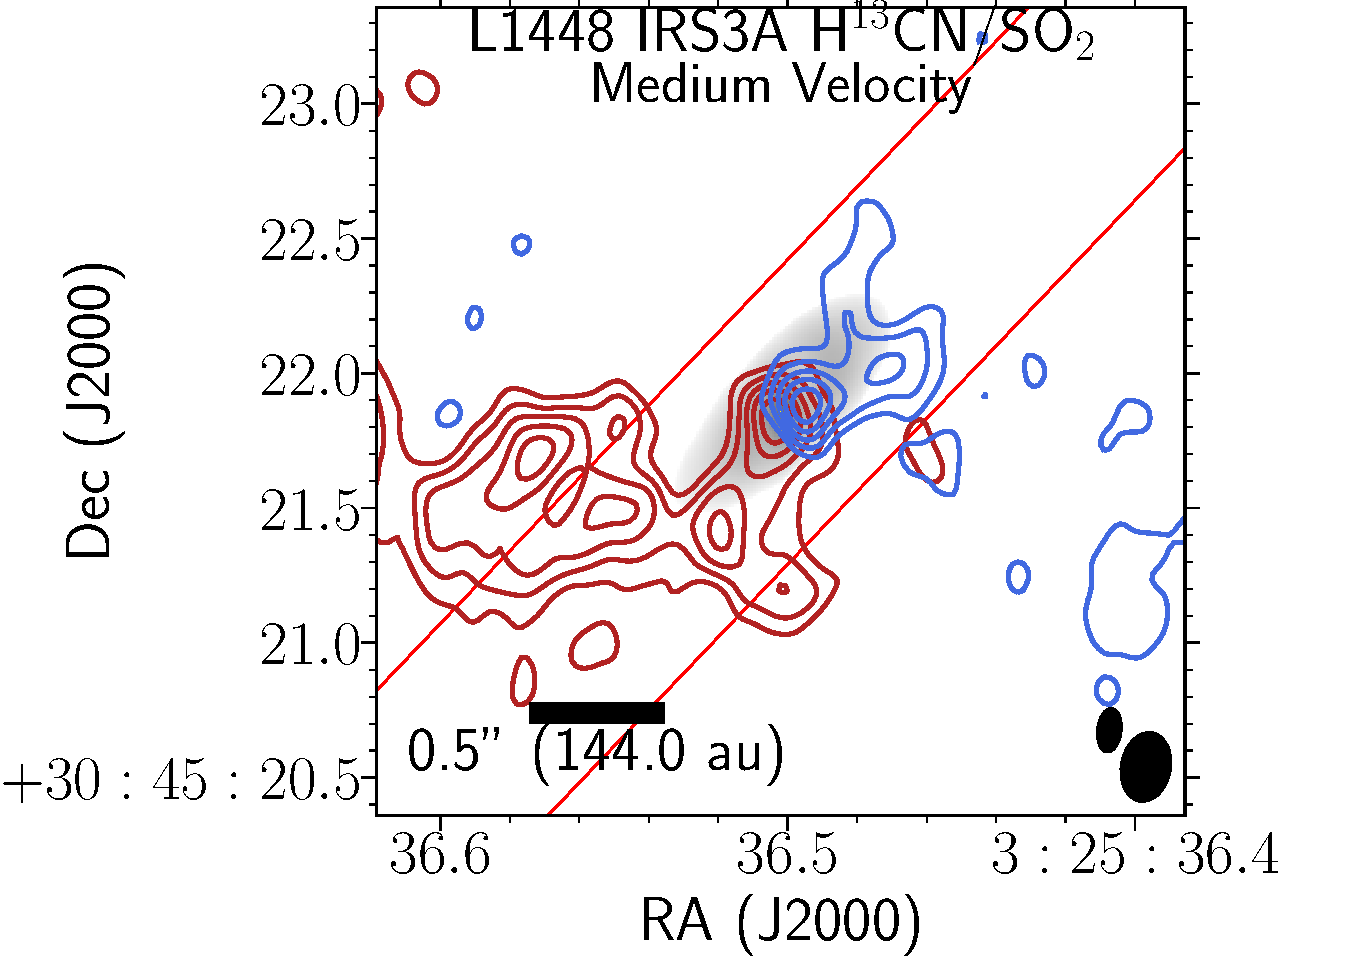
\includegraphics[width=0.33\textwidth]{img/L1448IRS3B_H13CN_image_taper1000k__-irs3amed_irs3a.pdf}
   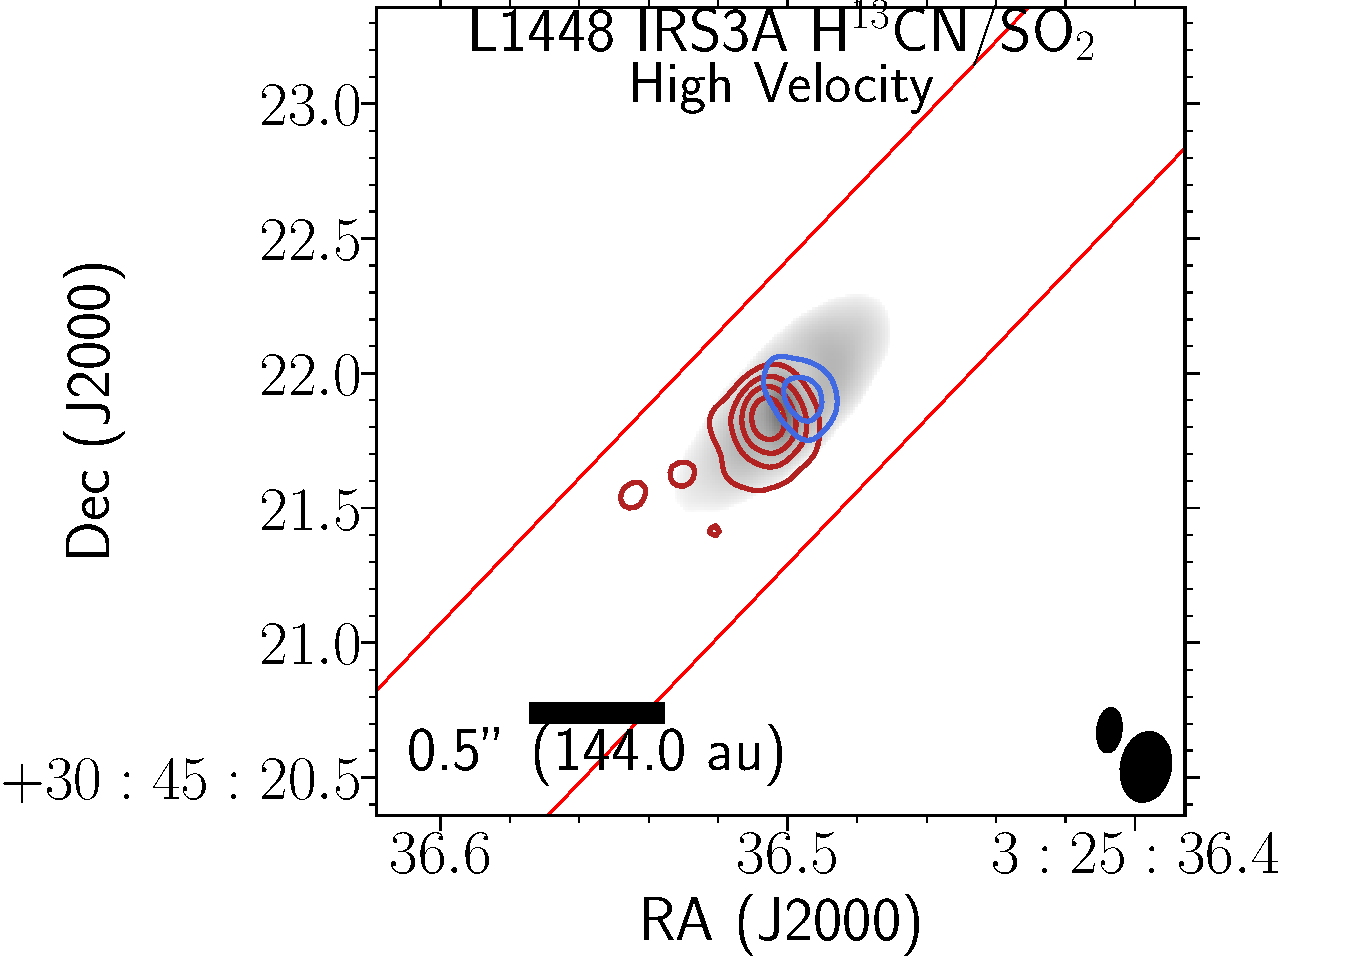
\includegraphics[width=0.33\textwidth]{img/L1448IRS3B_H13CN_image_taper1000k__-irs3ahigh_irs3a.pdf} % h13cn
\end{center}
   \caption{\htcn/\sot\space moment 0 map towards IRS3A; whose emission appears to trace rotation within the inner disk. The panels correspond to low, medium, and high velocity ranges which are delineated as red(blue), respectively. The system velocity of the \htcn/\sot\space emission (\ab5.4~km~s$^{-1}$) agrees with system velocity of \cso\space, likely tracing \htcn\space emission and not \sot\space emission. \textbf{Low Velocity:} velocity ranges 5.2$\rightarrow$6.5~\kms (4.1$\rightarrow$5.2~\kms), contours start at 4(4)$\sigma$ and iterate by 2(2)$\sigma$ with the 1$\sigma$~level starting at 0.0021(0.0021)~Jy~beam$^{-1}$ for the red(blue) channels respectively. \textbf{Medium Velocity:}  velocity ranges 6.5$\rightarrow$7.4~\kms (3.0$\rightarrow$4.1~\kms), contours start at 4(4)$\sigma$ and iterate by 2(2)$\sigma$ with the 1$\sigma$~level starting at 0.0016(0.0016)~Jy~beam$^{-1}$ for the red (blue) channels respectively. \textbf{High Velocity:} velocity ranges 7.4$\rightarrow$8.6~\kms (1.8$\rightarrow$3.0~\kms), contours start at 4(4)$\sigma$ and iterate by 3(3)$\sigma$ with the 1$\sigma$~level starting at 0.0021(0.0021)~Jy~beam$^{-1}$ for the red(blue) channels respectively. The \htcn\space synthesized beam (\htcnbeam) is the bottom-right most ellipse on each of the panels and the continuum synthesized beam (\contbeam) is offset diagonally.}\label{fig:irs3ah13cnmoment}
\end{figure}


% Figure 9
\begin{figure}[H]
\begin{center}
   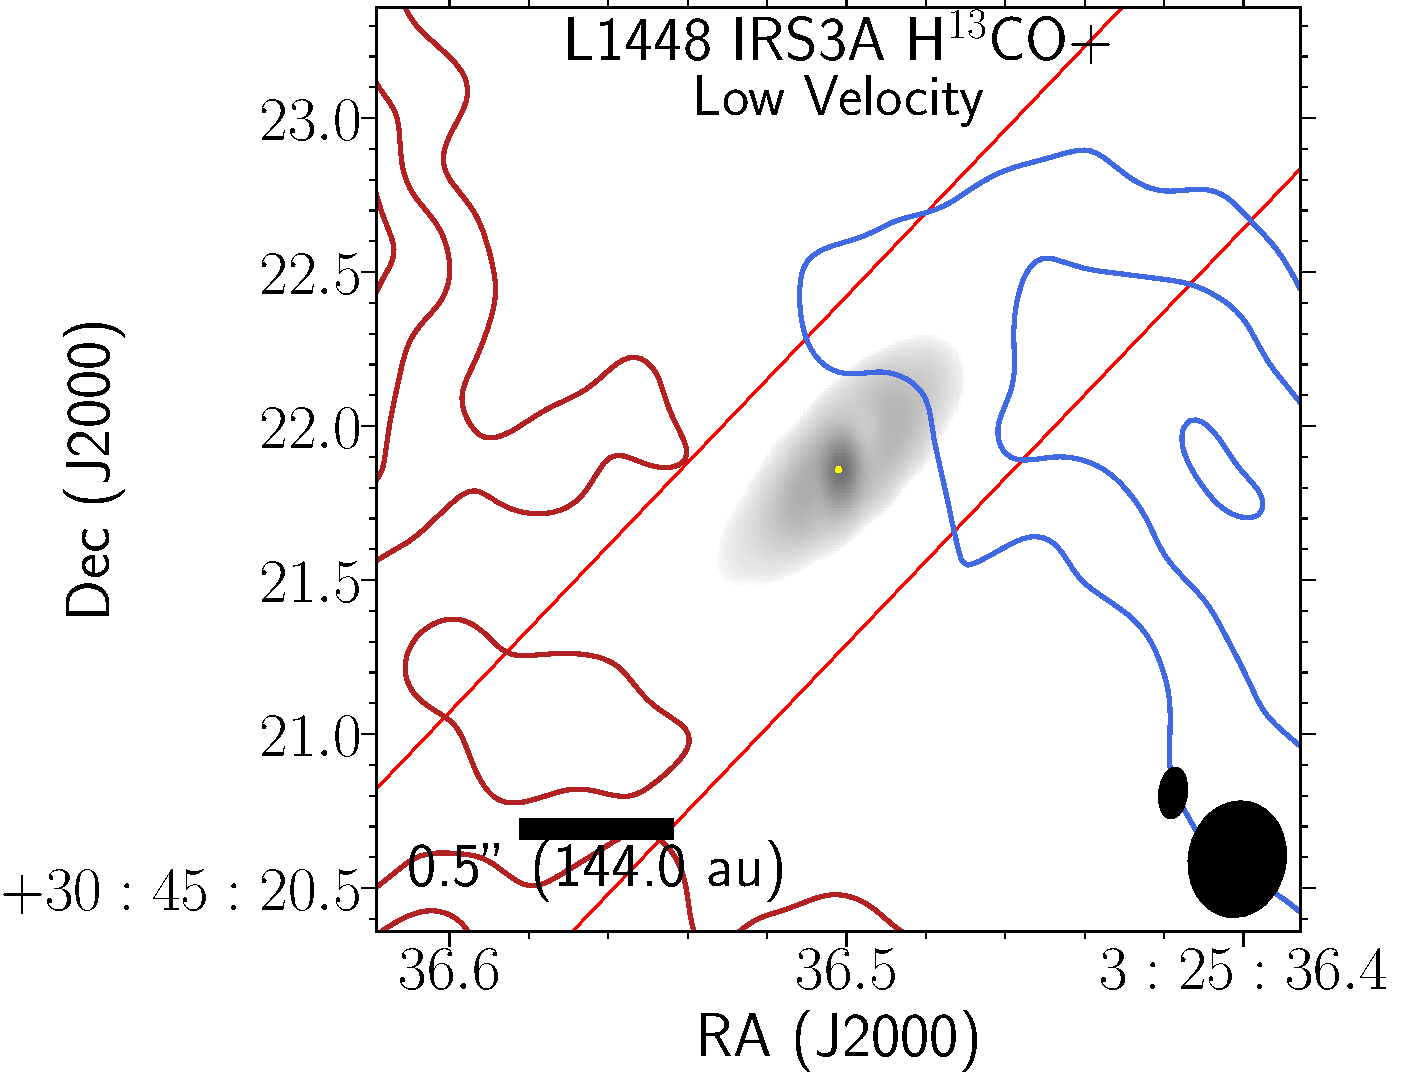
\includegraphics[width=0.33\textwidth]{img/L1448IRS3B_H13COp_image_taper400k__low-irs3a.pdf}
   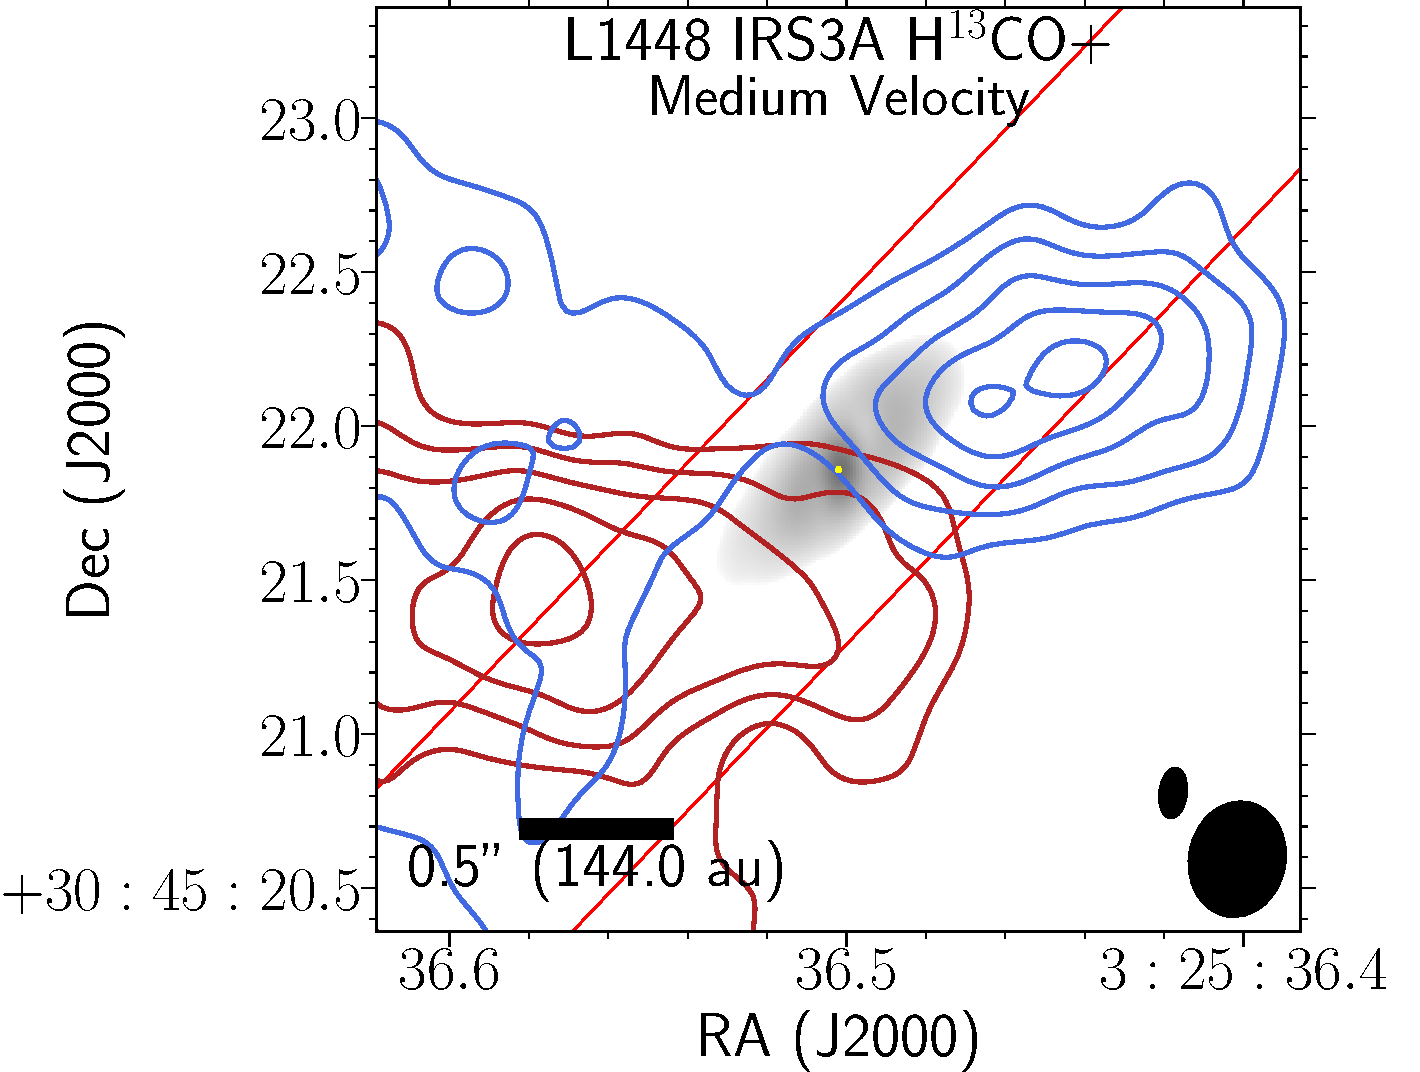
\includegraphics[width=0.33\textwidth]{img/L1448IRS3B_H13COp_image_taper400k__medium-irs3a.pdf}
   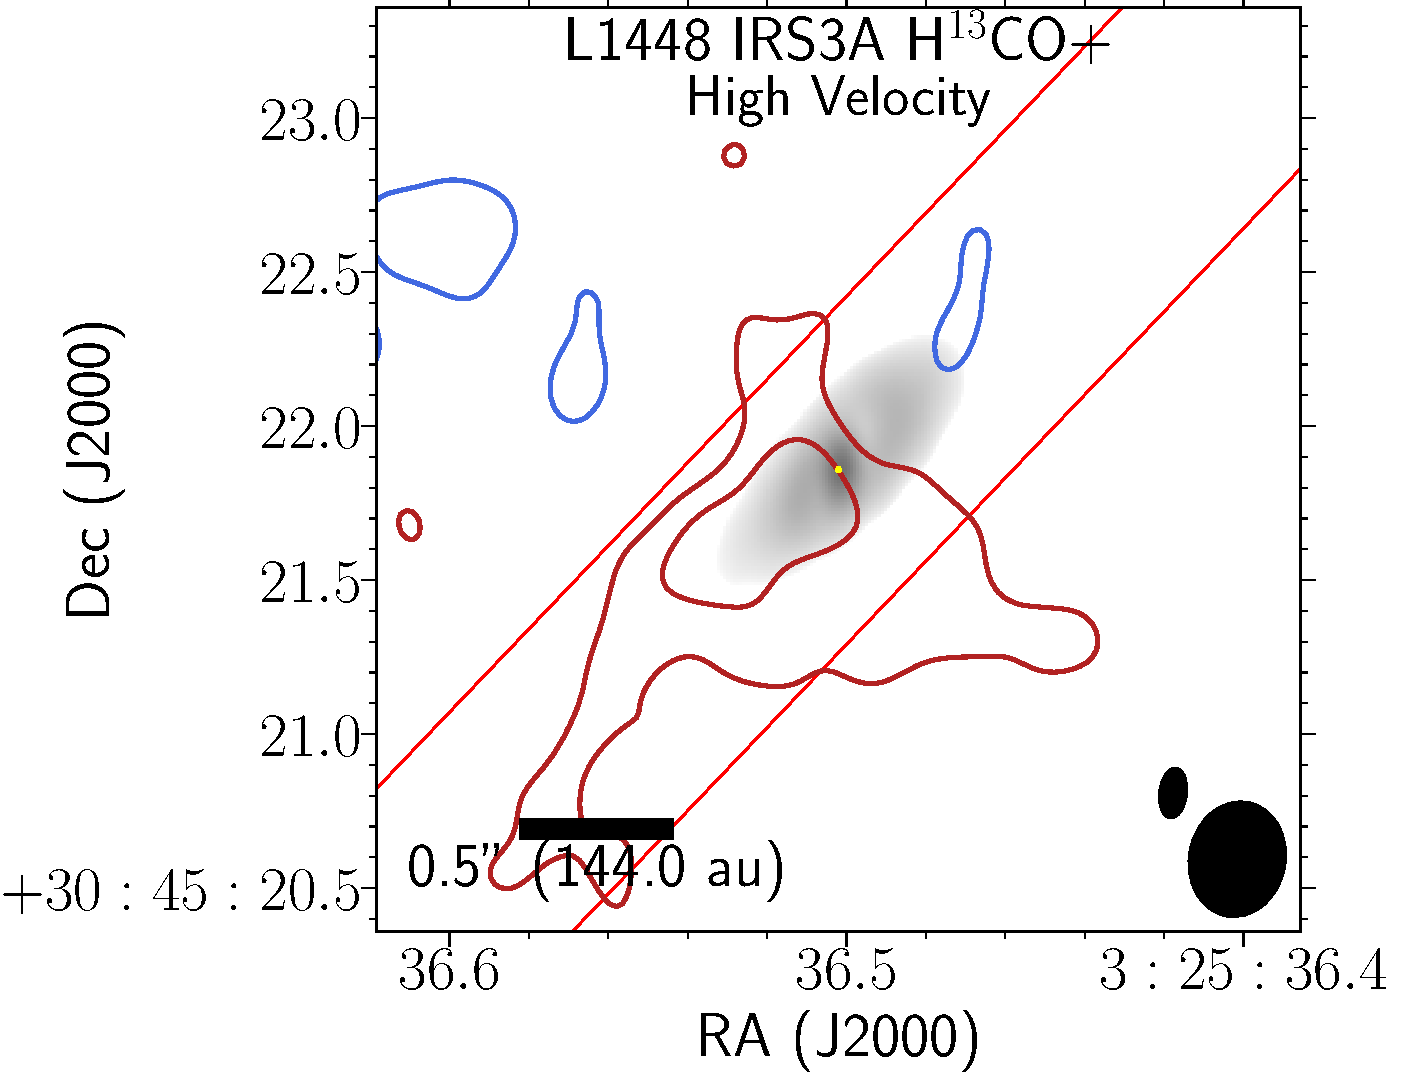
\includegraphics[width=0.33\textwidth]{img/L1448IRS3B_H13COp_image_taper400k__high-irs3a.pdf} % h13cn
\end{center}
   \caption{\htcop\space moment 0 map towards IRS3A. The image is tapered with a 400~k$\lambda$\space Gaussian. The \htcop\space emission might trace a velocity gradient across the source, but the lack of strong emission coming from the disk itself hinders resolving the kinematics. The columns correspond to low, medium, and high velocity ranges. \textbf{Low Velocity:} velocity ranges 5.2$\rightarrow$6.5~\kms (4.1$\rightarrow$5.2~\kms), contours start at 5(5)$\sigma$ and iterate by 2(2)$\sigma$ with the 1$\sigma$~level starting at 0.004(0.007)~Jy~beam$^{-1}$ for the red(blue) channels respectively. \textbf{Medium Velocity:}  velocity ranges 6.5$\rightarrow$7.4~\kms (3.0$\rightarrow$4.1~\kms), contours start at 3(3)$\sigma$ and iterate by 2(2)$\sigma$ with the 1$\sigma$~level starting at 0.003(0.003)~Jy~beam$^{-1}$ for the red (blue) channels respectively. \textbf{High Velocity:} velocity ranges 7.4$\rightarrow$8.6~\kms (1.8$\rightarrow$3.0~\kms), contours start at 3(3)$\sigma$ and iterate by 2(2)$\sigma$ with the 1$\sigma$~level starting at 0.002(0.0025)~Jy~beam$^{-1}$ for the red(blue) channels respectively. The \htcop\space synthesized beam (\htcopbeam) is the bottom-right most ellipse on each of the panels and the continuum synthesized beam (\contbeam) is offset diagonally.}\label{fig:irs3ah13copmoment}
\end{figure}

% Figure 4
\begin{figure}[H]
\begin{center} % c17o
   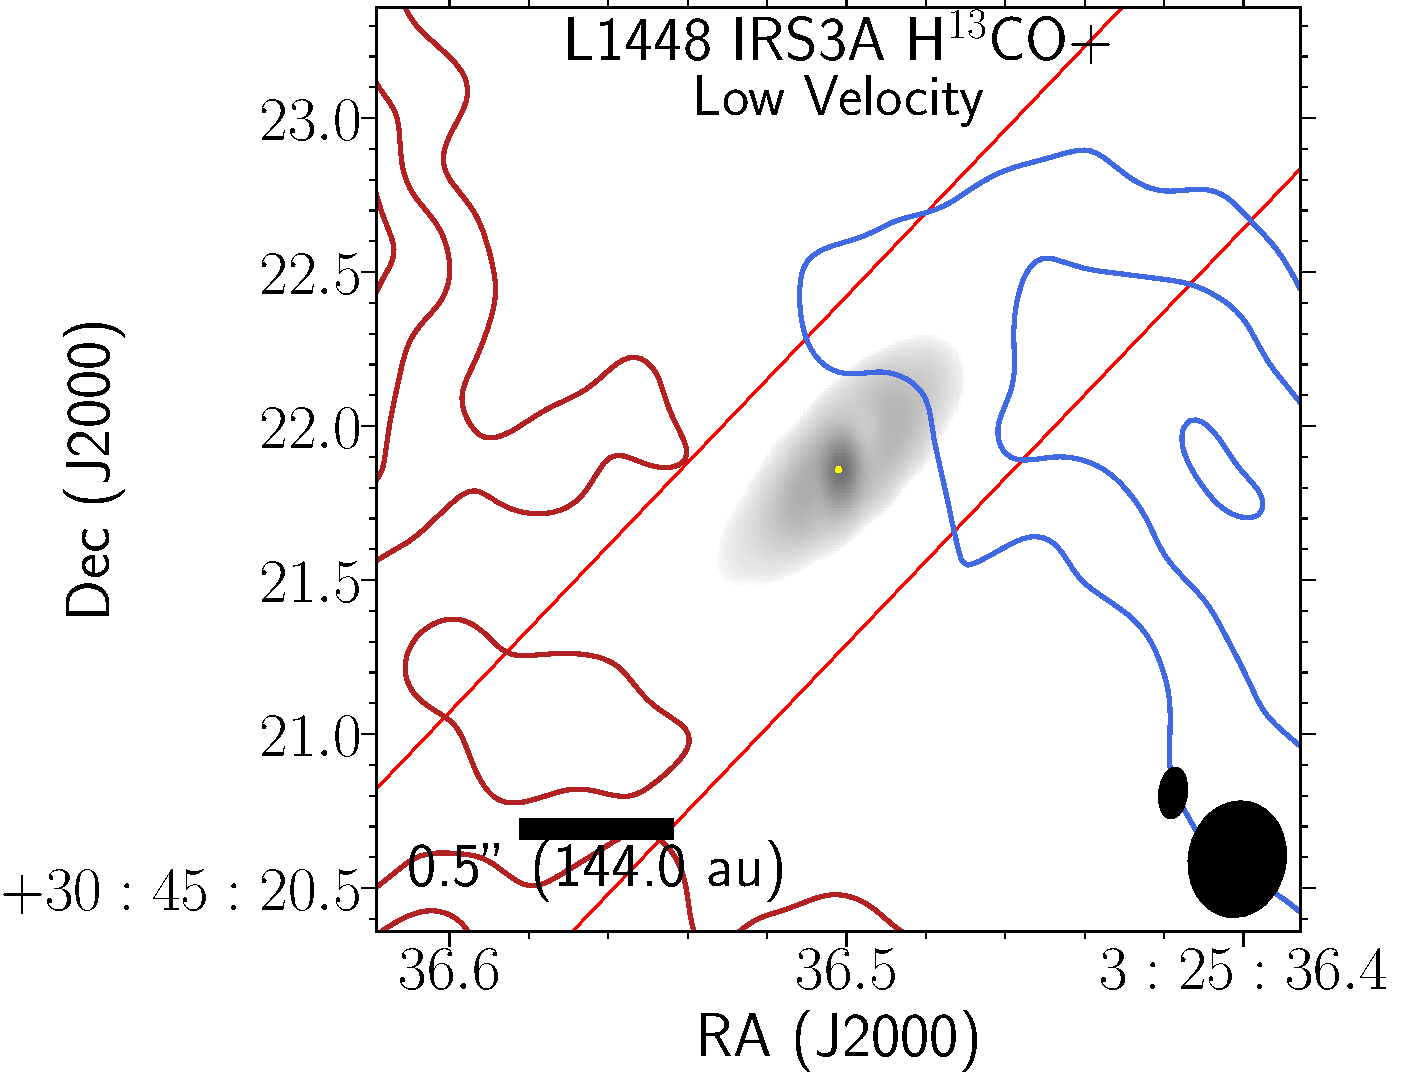
\includegraphics[width=0.33\textwidth]{img/L1448IRS3B_H13COp_image_taper400k__low.pdf}
   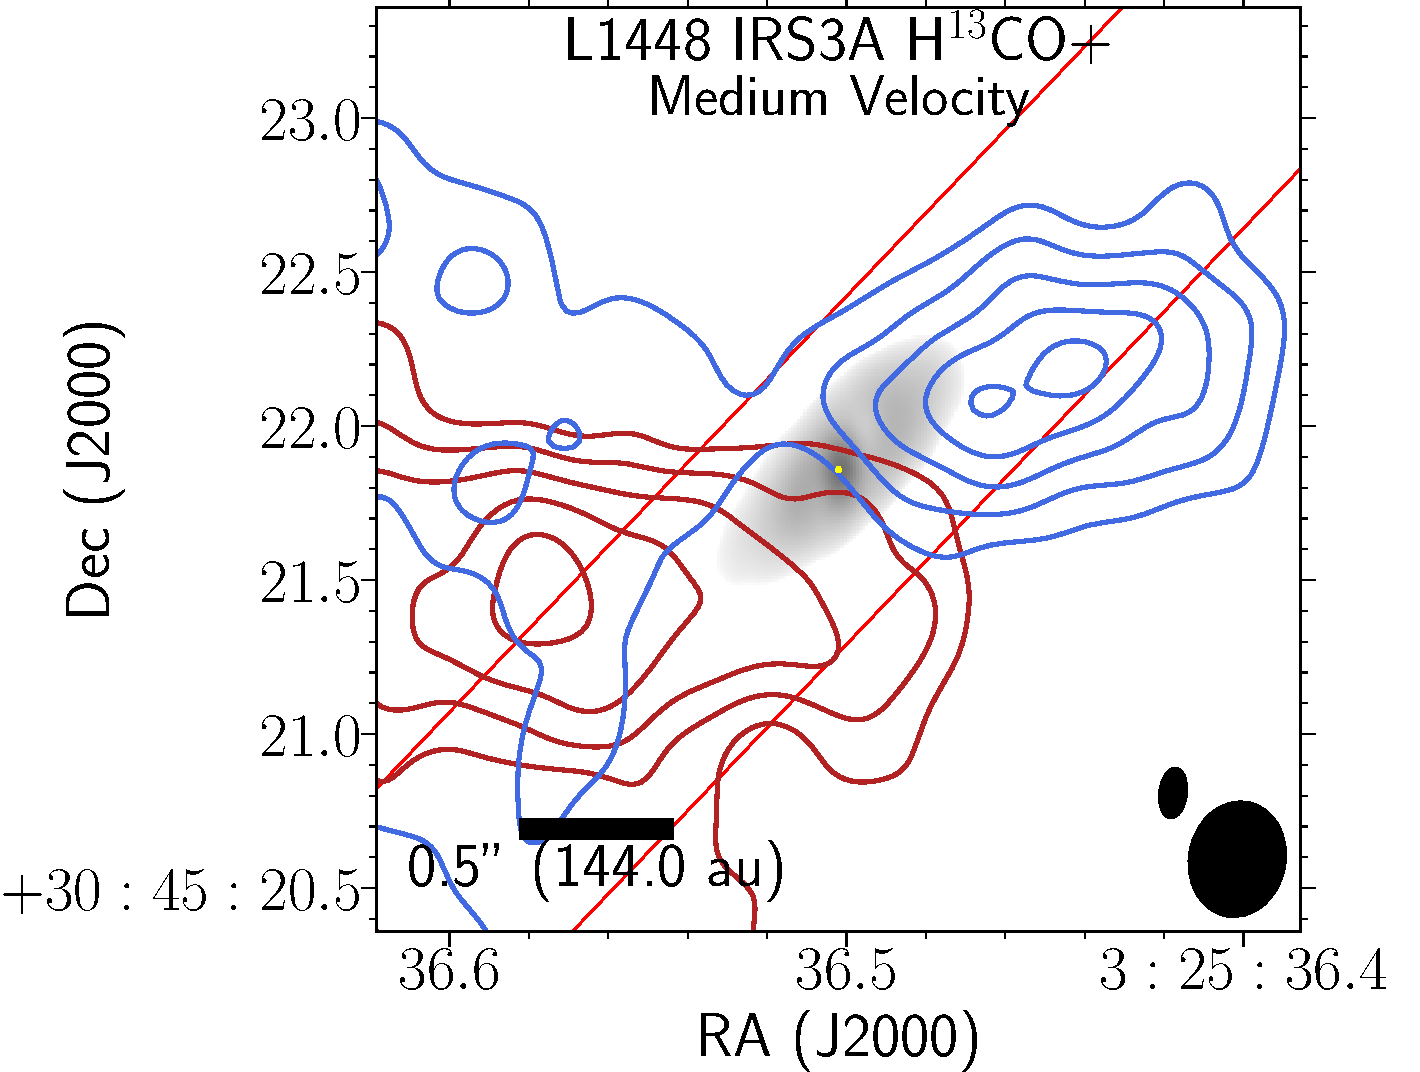
\includegraphics[width=0.33\textwidth]{img/L1448IRS3B_H13COp_image_taper400k__medium.pdf}
   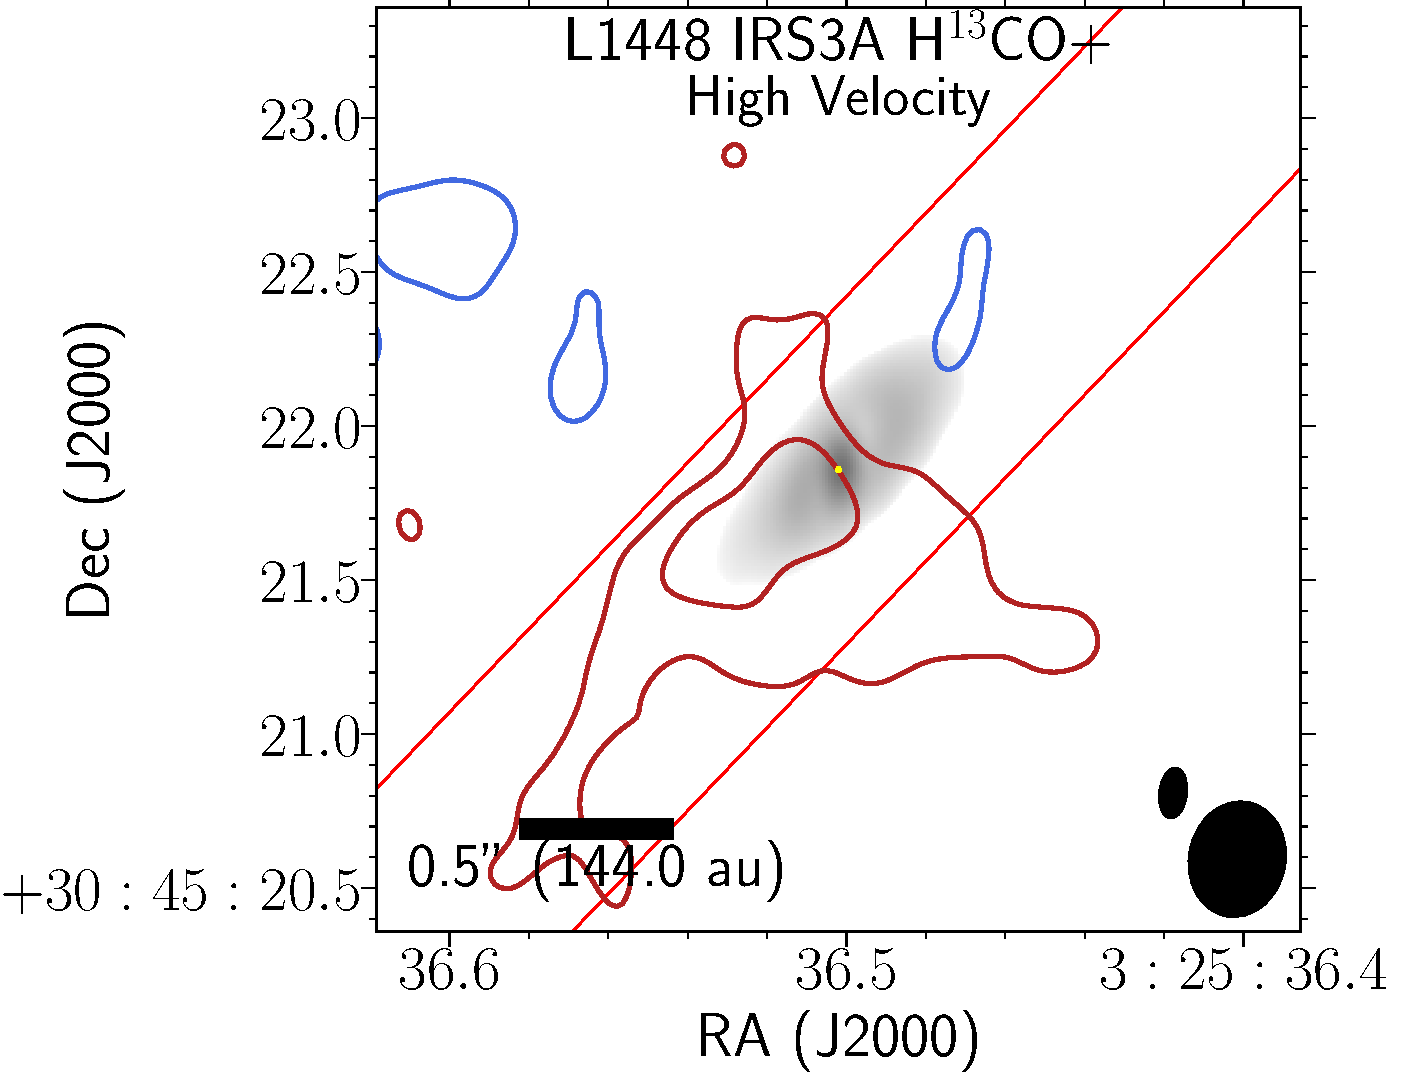
\includegraphics[width=0.33\textwidth]{img/L1448IRS3B_H13COp_image_taper400k__high.pdf}
\end{center}
   \caption{Similar image to Figure~\ref{fig:irs3bc17omoment}\space towards IRS3B but with \htcop. The top row spatial scale is set to match those of Figure~\ref{fig:irs3bc17omoment} and the bottom row scale is set to encapsulate the entire IRS3B system, to better demonstrate the spatial scales probed with this molecule. The top row is tapered with a 400~k$\lambda$\space Gaussian to best reduce the amount of noise and show the proper resolution to the spatial scales shown. The columns correspond to similar velocity ranges of \cso. The red lines indicate the region extracted for PV diagram construction, along the position angle of the major axis in a region much larger than the \cso\space PV diagram extraction to fully capture the emission. \textbf{Low Velocity:} contours start at 10(10)$\sigma$ and iterate by 2(2)$\sigma$ with the 1$\sigma$~level starting at 0.003(0.003)~Jy~beam$^{-1}$ for the top row and 0.005(0.005)~Jy~beam$^{-1}$ for the bottom row,  red(blue) channels respectively.  \textbf{Medium Velocity:}  contours start at 5(5)$\sigma$ and iterate by 5(3)$\sigma$ with the 1$\sigma$~level starting at 0.005(0.005)~Jy~beam$^{-1}$ for the top row and 0.005(0.005)~Jy~beam$^{-1}$ for the bottom row, red(blue) channels respectively. \textbf{High Velocity:} contours start at 5(5)$\sigma$ and iterate by 2(2)$\sigma$ with the 1$\sigma$~level starting at 0.002(0.002)~Jy~beam$^{-1}$ for the top row and 0.005(0.005)~Jy~beam$^{-1}$ for the bottom row, for the red(blue) channels respectively. The \htcop\space synthesized beam (top:0\farcs374$\times$0\farcs310, bottom: \htcopbeam) is the bottom-right most ellipse on each of the panels and the continuum synthesized beam (\contbeam) is offset diagonally.}\label{fig:h13copmomentc17o}
\end{figure}



% Figure 8
% irs3a
\begin{figure}[H]
\begin{center}
   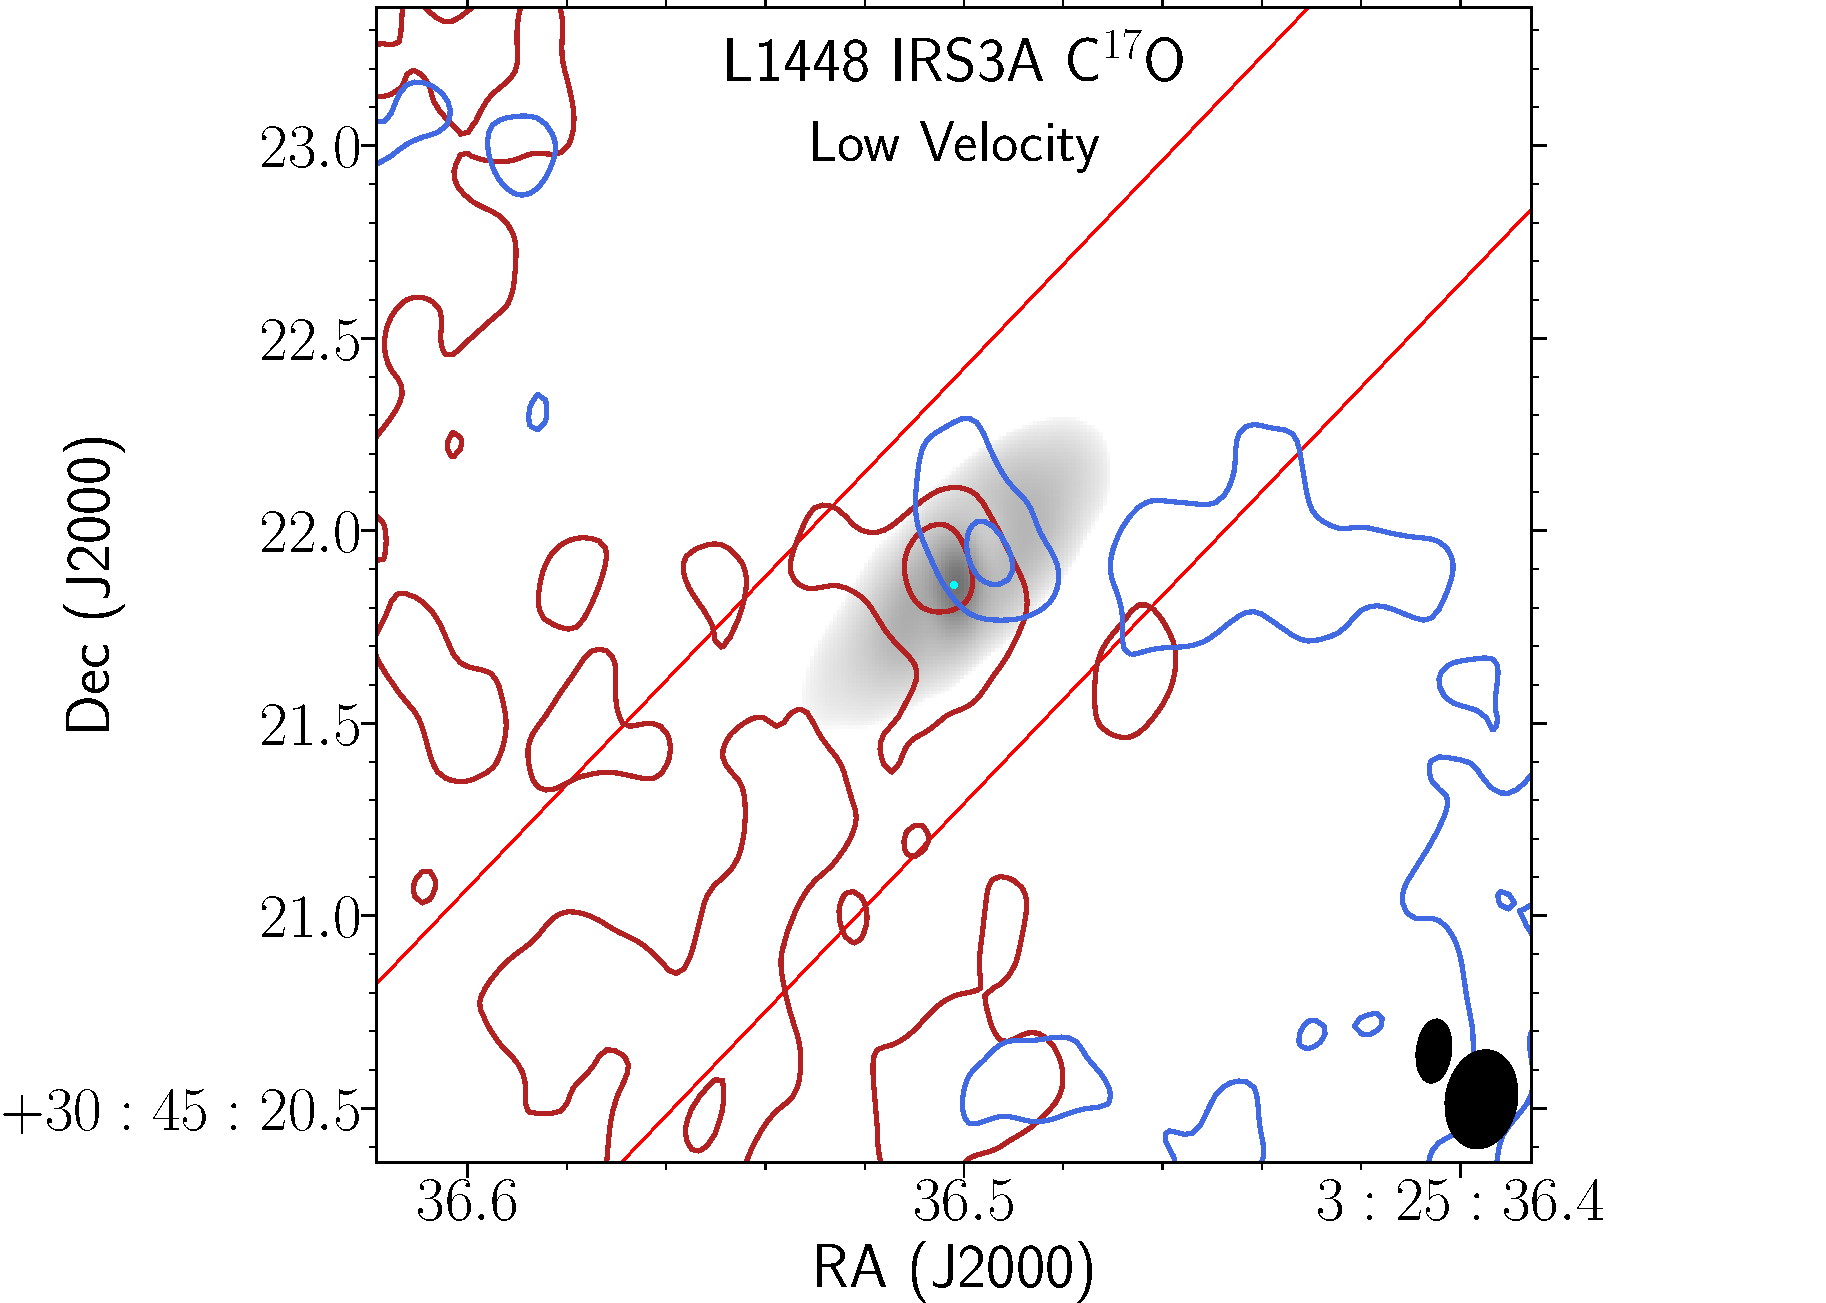
\includegraphics[width=0.33\textwidth]{img/L1448IRS3B_C17O_image_taper1500k__-irs3asplitMoments_low_irs3a.pdf}
   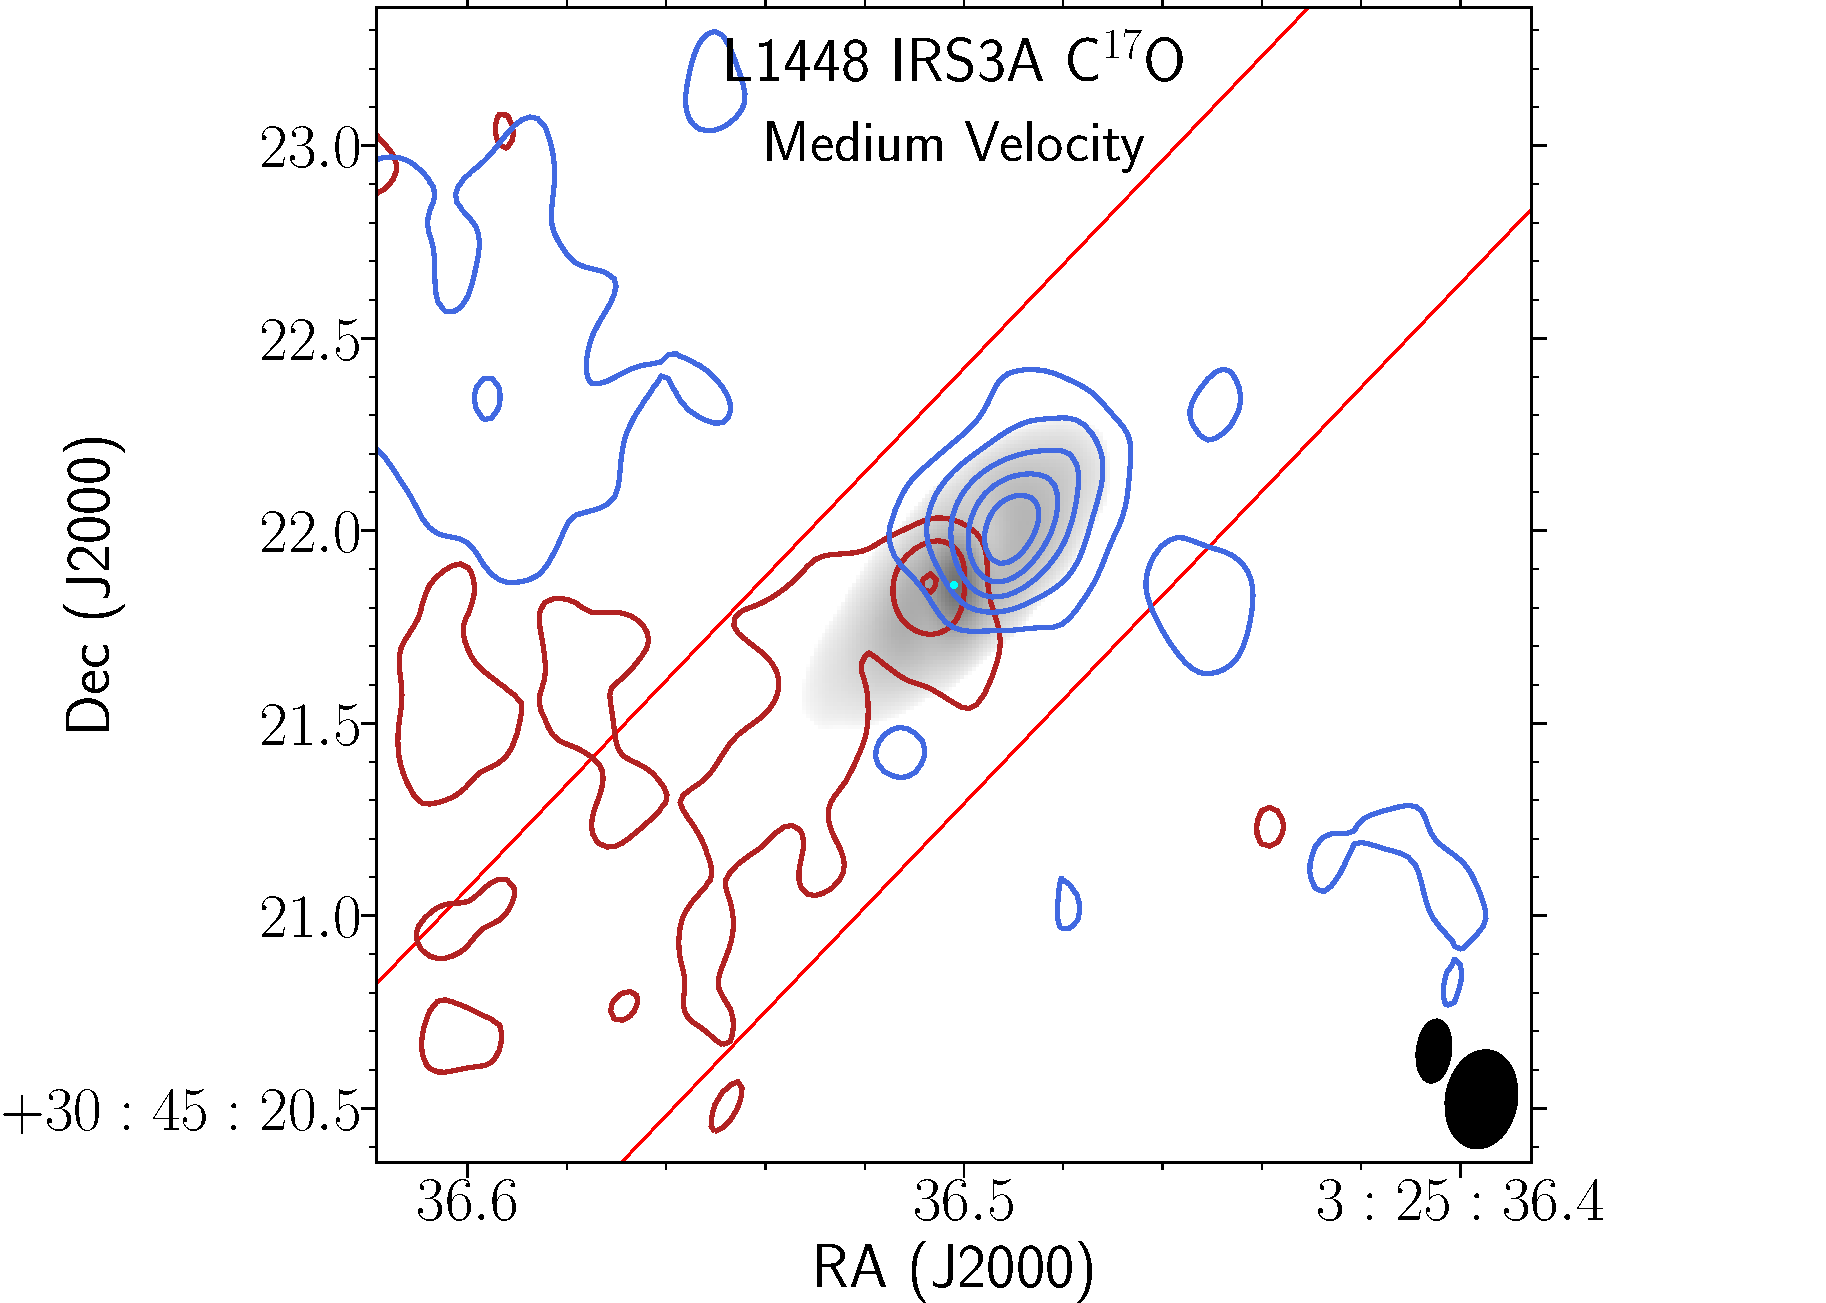
\includegraphics[width=0.33\textwidth]{img/L1448IRS3B_C17O_image_taper1500k__-irs3asplitMoments_med_irs3a.pdf}
   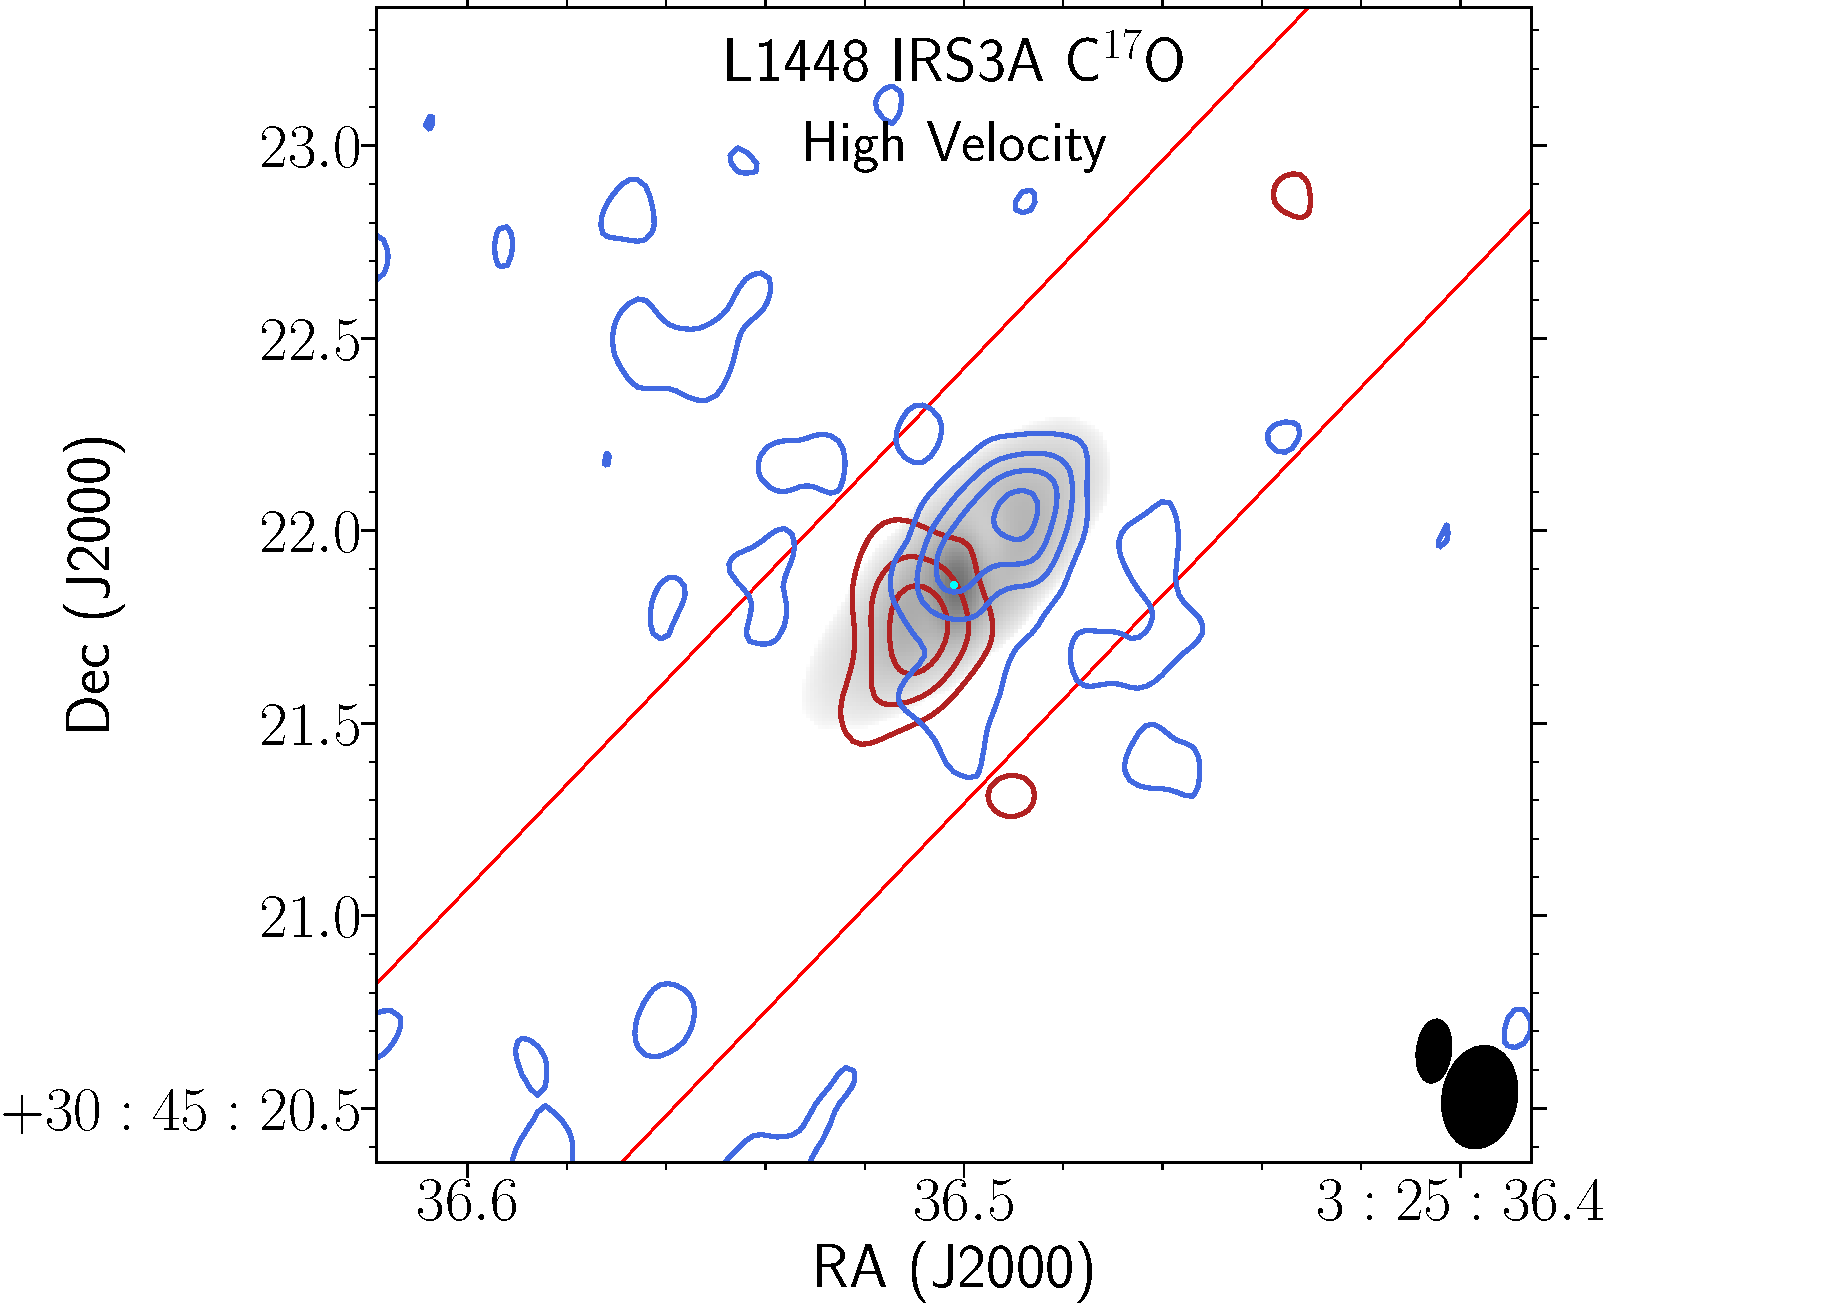
\includegraphics[width=0.33\textwidth]{img/L1448IRS3B_C17O_image_taper1500k__-irs3asplitMoments_high_irs3a.pdf} 
\end{center}
   \caption{Similar image to Figure~\ref{fig:irs3bc17omoment}\space towards IRS3A. However, S/N is low in comparison to IRS3B. \textbf{Low Velocity:} velocity ranges 5.2$\rightarrow$6.5~\kms (4.1$\rightarrow$5.2~\kms), contours start at 3(3)$\sigma$ and iterate by 3(3)$\sigma$ with the 1$\sigma$~level starting at 0.0023(0.0025)~Jy~beam$^{-1}$ for the red(blue) channels respectively. \textbf{Medium Velocity:}  velocity ranges 6.5$\rightarrow$7.4~\kms (3.0$\rightarrow$4.1~\kms), contours start at 3(3)$\sigma$ and iterate by 3(3)$\sigma$ with the 1$\sigma$~level starting at 0.002(0.0016)~Jy~beam$^{-1}$ for the red (blue) channels respectively. \textbf{High Velocity:} velocity ranges 7.4$\rightarrow$8.6~\kms (1.8$\rightarrow$3.0~\kms), contours start at 3(3)$\sigma$ and iterate by 3(3)$\sigma$ with the 1$\sigma$~level starting at 0.0018(0.0012)~Jy~beam$^{-1}$ for the red(blue) channels respectively. The \cso\space synthesized beam (\csobeam) is the bottom-right most ellipse on each of the panels and the continuum synthesized beam (\contbeam) is offset diagonally.}\label{fig:irs3ac17omoment}
\end{figure}




